\documentclass{../../template/esiwace-report}


%%%%%%%%%%%%%%%%%%%%%%%%%%%%%%%%%%%%%%%%%%%%%%%%%%%%%%%%%%%%%%%%%%%%%%%%%%%%%%%
%%%%%%%%%%%%%%%%%%%%%%%%%%%%%%%%%%%%%%%%%%%%%%%%%%%%%%%%%%%%%%%%%%%%%%%%%%%%%%%
\title{D4.2 New Storage Layout for Earth System Data}
\author{Jakob Lüttgau 
\and Julian Kunkel
\and Bryan Lawrence
\and Jens Jensen
\and Giuseppe Congiu
}
	
\date{\today} % Replace with final date

\ESIWACEworkpackage{WP4 Exploitability}
\ESIWACElead{DKRZ}
\ESIWACEparticipants{Seagate, CMCC, STFC, ECMWF}

\usepackage{adjustbox}


\begin{document}
\maketitle
%%%%%%%%%%%%%%%%%%%%%%%%%%%%%%%%%%%%%%%%%%%%%%%%%%%%%%%%%%%%%%%%%%%%%%%%%%%%%%%
%%%%%%%%%%%%%%%%%%%%%%%%%%%%%%%%%%%%%%%%%%%%%%%%%%%%%%%%%%%%%%%%%%%%%%%%%%%%%%%
\begin{abstract}
Making the best use of HPC in Earth simulation requires storing and manipulating vast quantities of data.
Existing storage environments face usability and performance challenges for both domain scientists and the data centers supporting the scientists.
%These obstacles stem from ideas implied by POSIX file systems and external data services.
These challenges arise from data discovery/access patterns, and the need to support complex legacy interfaces.
In the ESiWACE project, we develop a novel I/O middleware targeting, but not limited to, earth system data.
This deliverable sheds light upon the technical design of the ESD middleware, and the user perspective and implications when using the middleware.
Its architecture builds on well established end-user interfaces but utilizes scientific metadata to harness a data structure centric perspective. 

In contrast to existing solutions, the middleware maps data structures to available storage technology based on several parameters:
1) A data center specific configuration of available hardware with their characteristics;
2) The intended usage pattern explicitly provided by the user and implicitly by the structure of the data.

This allows to exploit performance characteristics of a heterogeneous storage environment more efficiently.
\end{abstract}
%%%%%%%%%%%%%%%%%%%%%%%%%%%%%%%%%%%%%%%%%%%%%%%%%%%%%%%%%%%%%%%%%%%%%%%%%%%%%%%
%%%%%%%%%%%%%%%%%%%%%%%%%%%%%%%%%%%%%%%%%%%%%%%%%%%%%%%%%%%%%%%%%%%%%%%%%%%%%%%
% #####  ###    ###
%   #   #   #  #
%   #    ###    ###
\newpage
\tableofcontents
\newpage
%%%%%%%%%%%%%%%%%%%%%%%%%%%%%%%%%%%%%%%%%%%%%%%%%%%%%%%%%%%%%%%%%%%%%%%%%%%%%%%
%%%%%%%%%%%%%%%%%%%%%%%%%%%%%%%%%%%%%%%%%%%%%%%%%%%%%%%%%%%%%%%%%%%%%%%%%%%%%%%
\chapter{Relation to the Project}
% Description of the task / WP / Deliverable.
% Copy the text of the proposal here and add some filling to make sure people can understand.

The following text is the description of the project proposal for this task and deliverable:

\begin{quote}
\itshape
%Developing a New disk storage layout for Earth system data to overcome the performance limitations of existing fixed on-disk formats and APIs by providing a novel data-specific layout interface. The new interface will be capable of supporting both interoperability between higher-level file formats and of customisation to local heterogeneous disk storage environments.

I/O is being addressed at a number of levels within ESiWACE, since both current experience
and projections have highlighted the performance/volume challenges ahead.
The main goal of this task is to address performance and physical capacity issues associated with
writing, accessing, and earth system data in the disk subsystem themselves.
One key problem that can be addressed is separation of file metadata operations from the data access -
this is the strategy some hybrid disk systems use to improve performance by putting file system metadata on SSD and data itself on spinning platters.
However, with netCDF or GRIB data, the scientific relevant metadata and much of the information about actual data layout is invisible to the file system (whether parallel or serial), which cannot then exploit acceleration techniques.
To address this, we propose and test an Earth System Data (ESD) middleware library which understands these key formats, and which is customizable for different hardware environments (as will occur in differing data center architectures).
It will support, for example, writing the scientific metadata and possibly coordinate access to SSD systems, and the binary data fields to traditional systems potentially split into multiple files.
Where in-memory storage backends are available, fast online data analytics will also become possible.
[...]
%The architecture is illustrated in the Figure below.
The layout components will decide the data placement and orchestrate data access on the storage characteristics.
But blocking and non-blocking APIs will be supported to address typical use-cases.
Tools will accompany the library so that data can be reconstructed as compatible with netCDF/GRIB and can be archived and exchanged.
\end{quote}




%%%%%%%%%%%%%%%%%%%%%%%%%%%%%%%%%%%%%%%%%%%%%%%%%%%%%%%%%%%%%%%%%%%%%%%%%%%%%%%
%%%%%%%%%%%%%%%%%%%%%%%%%%%%%%%%%%%%%%%%%%%%%%%%%%%%%%%%%%%%%%%%%%%%%%%%%%%%%%%
\chapter{Introduction}

\begin{chapterIntro}
This section motivates the development of the new middleware and lists the challenges specifically for Numerical Weather Prediction (NWP) and climate.
\end{chapterIntro}

\section{Motivation}

The development of the new middleware is motivated by two facts:

\begin{enumerate}
	\item Firstly, the drastic changes in the storage landscape.
	\item Secondly, the drawbacks of the current data management paradigm.
\end{enumerate}


\subsection{Changes in the Storage Landscape}

With the emergence of new storage technologies such as NVRAM and cloud storage, the sea of options for storing data becomes increasingly complex.
The storage architecture of novel systems deploys combinations of several technologies as a single solution. This is motivated by the fact that systems
relying only on hard disk drives (HDDs) cannot deal with all the workloads efficiently. On the other hand, building systems that can serve different 
workloads by dynamically directing them to the storage media that serves their need best, can provide a better solution although it increases complexity.

\todo{Refer to outcomes of cost discussions (JJ: is this enough?)}
Deliverable D4.1 investigated models for the data centre, focusing on the cost of providing services of the required QoS, e.g. with the required durability qualities, availabilities, etc.; in particular, services could be made up of different types of storage, and in general different kinds of storage are required also to support the processing of the data (e.g. scratch space, archiving, working repositories, space to share with other users, etc.)  As climate and weather data volumes scale up, one needs to investigate which parts of the data centre and its operation need to scale up, and by how much.  For example, operating the first tape library requires employing and training staff to look after it, but then operating another tape library does not require double the staff.  Support for the users, though, is expected to scale approximately linearly with the number of users.

In particular, different types of services are needed to support different parts of the data processing -- storage, archiving, possibly preservation, cache, fast disk for HPC/HTC, etc.  No single storage ``solution'' meets all these requirements.  Thus, systems consisting of multiple storage technologies are combined to provide various services, traditionally in a memory hierarchy, because fast and expensive devices come
with less capacity than slow and cheap(er) devices.  Fast disk can then cache ``hot'' files which are being processed by many jobs, and slower storage with higher capacity can manage the rest of the data.

On many systems, data migration from one persistent storage hierarchy to another, e.g., disk based scratch to long term tape, is initiated by the user.
This is an inconvenient additional step for the user but gives explicit knowledge about the data location. Depending on the usage, this may lead to a more efficient 
exploitation of the near-line storage, but only for educated users that know their workflow well.

An hierarchical storage system (HSM) extends this notion allowing administrators to define policies that describe how data is placed and potentially migrated between 
different storage tiers. However, HSMs operate at the file granularity (according to the definition of file systems). Block-based data migration can also be supported
by some system. Both approaches have in common that they do not understand the data structures that are serialized to the 1D Byte array of a file.

Also the increasing use of object storage is relevant to this report.  Currently, there are activities looking at the placements of slices of multidimensional HDF5 arrays into object stores, with a unified addressing and lazy loading in applications.  Provided data is being indexed correctly, optimised storage of larger arrays can lead to a speed-up of processing of two orders of magnitude, so it will be worth investigating this topic further.

\subsection{Data Management Paradigm}

The file based data management paradigm forces users to define the hierarchical namespace in which store the experiments.
From the user perspective, scientific file formats could store one or multiple variables in one file, which can be potentially partitioned and distributed across 
multiple physical files. Usually, the definition of the content of a file is driven by performance reasons and the initial originating process (i.e., the scientific 
program generating the data). In many cases, a portable data format that can be used to exchange data between working groups and scientists, is another important factor. 
However, a file format may not optimally support the workload or the storage system it is running on. The users could struggle to define a file system hierarchy that matches 
their workflow and is well performing on their system; indeed, some user communities overload the file paths with metadata to aid its discovery, but this also does not scale in the general case.

Once all data is ready, usually scientific databases are used to ingest the metadata and offer alternative views to the same data. They abstract from the actual 
hierarchical namespace used underneath and provide a flexible approach to query data.

\todo{More limitations later...}




\section{Challenges for NWP/Climate}

Workloads from the domain of climate and weather face particular challenges in terms of data management and storage landscape\footnote{Note that other scientific domains have some overlap with the mentioned challenges, in that sense none of the challenges is unique for NWP/climate but in the combination the profile is unique.}.

\begin{enumerate}
\item \textbf{I/O intensity (volume and velocity)}.
Multiple data sources can be used in one simulation or analysis.
Observational sources such as satellites and sensor networks can produce large volumes of data.
Simulations can produce data at any granularity: Firstly, the resolution can be increased. 
Secondly, ensemble runs as mixes of multiple scenarios, number of experiments to be conducted and, thus, the data volume.


\item \textbf{Code portability}. Code is long-living, it can potentially live for decades, and excerpts of the code might be moved to newer code.
Historically researchers used to optimize codes for specific supercomputers but with increasingly complex systems this approach is not feasible.
Thus, data management needs to scale with future data volumes in a way which provides acceptable data access latencies and data durability, and is cost-effective. 
In this context the middleware hides specifics of the storage landscape and does not require users to change parameters specifically to a given system.


\item \textbf{There is no single perfect model}. 
  The complexity of the physical processes that influence weather and climate is so immense that not all parameters are yet understood and can be quantified. 
  This leads to a proliferation of predictive models. Each of them covers the processes slightly differently or covers alternative processes. 
  Thus all of the models have some relevance and cannot be unified easily.

\item \textbf{Diversity of data formats and middleware}.
In an effort to allow for easier exchange and inter-comparison of model and observations, data libraries for standardized data description and optimized I/O such as NetCDF, HDF5 and GRIB were developed but many more legacy formats exist. Since historical data is important, these formats must still be supported and maintained.
Many I/O optimizations used in common libraries do not adequately reflect current data intensive system architectures, as they are maintained from domain scientists 
and not computer scientists.


\item \textbf{Sharing of data between many stakeholders}.
Systems need to support multi-disciplinary research through shared, interoperable interfaces, based on open standards and deliver environmentally-responsible and flexible hybrid data and compute infrastructures.

\item \textbf{Time critical and guaranteed accuracy are mandatory}. 
Climate and weather applications can be used for the prediction of disasters such as tsunamis.
This implies that the models must produce the well-defined and accurate output; and that in-situ and in-transit workflows are supported.
It is also crucial that the runtime of such a prediction is short to react accordingly and mitigate the impact on society.
\end{enumerate}


\section{Outline}

This deliverable is organized as follows:


\todo{}


%%%%%%%%%%%%%%%%%%%%%%%%%%%%%%%%%%%%%%%%%%%%%%%%%%%%%%%%%%%%%%%%%%%%%%%%%%%%%%%
%%%%%%%%%%%%%%%%%%%%%%%%%%%%%%%%%%%%%%%%%%%%%%%%%%%%%%%%%%%%%%%%%%%%%%%%%%%%%%%
\chapter{Earth System Data}

\begin{chapterIntro}
This chapter provides a high-level perspective on the data formats, middleware used for managing earth system data and how these are utilized by end-users and developers.
\end{chapterIntro}



\section{Data Generated by Simulations}

With the progress of computers and increase of observation data, numerical models were developed. 
A numerical weather/climate model is a mathematical representation of the earth’s climate system, that includes the atmosphere, oceans, landmasses and the cryosphere. 
The model consists of a set of grids with variables such as surface pressure, winds, temperature and humidity. 
A numerical model can be encoded in a programming language resulting in an application that simulates the behavior based on the model.
Inside an application, a grid is used to describe the covered surfaces of the model, which often is the globe.
Traditionally, the globe has been divided based on the longitude and latitude into rectangular boxes.
Since this produced unevenly sized boxes and singularities closer to the poles, modern climate applications use hexagonal and triangular meshes.
Particularly triangular meshes have an additional advantage, that one can refine regions and, thus, can decide on the granularity that is needed locally -- this leads to numeric approaches of the multi-grid methods.
Grids that follow a regular pattern such as rectangular boxes or simple hexagonal grids are called structured grids. 
With partially refined grids or when covering complex shapes instead of the globe, the grids become unstructured, as they form an irregular pattern.

To create an hexagonal or triangular grid from the surface of the earth, the grid can be constructed starting from an icosahedron and repetitively refining the triangle faces until a desired resolution is reached.
Variables contain data that can either describes a single value for each cell, the edges of the cells, or the vertices of the cells.

\Cref{fig:grid} shows this localization -- the scope of data -- for the triangular and hexagonal grids.

\begin{figure}[tb]
  \centering
  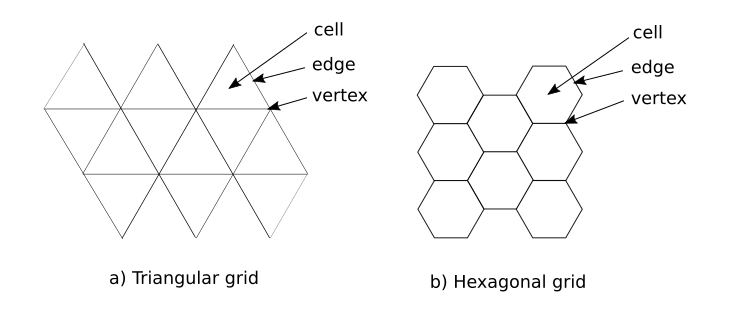
\includegraphics[width=.7\linewidth,natwidth=729,natheight=316]{hgrid.jpg}
  \caption{Scope of variables inside the grids}
  \label{fig:grid}
\end{figure}

Larger grids are shown in \Cref{fig:triangulargrid} and in (\Cref{fig:hexagonalgrid}).
There are figures provided that illustrate the neighborhood between data points and for different data localization.

\paragraph{Triangular grid} consists of cells shaped as a triangle (\Cref{fig:grid-triangleempty}). 
%It's structure is similar to hexagonal grid. 
Values can be located at the centers of the primal grid hexagons \Cref{fig:grid-trianglecenter}, and if we connect it to each other, we would see the grid of triangles \Cref{fig:grid-trianglecenter_derived}.
If values are located at the edes (\Cref{fig:grid-triangleedges}) and they are connected with its neighbours, then the grid will be seen \Cref{fig:grid-triangleedges_derived}.
If the values are located at the vertices and they are connected with its neighbours, then the grid will be seen in \Cref{fig:grid-trianglevertex}.

\paragraph{Hexagonal grid} consists of cells shaped as a flat topped hexagon (\Cref{fig:grid-hex-empty}).
Two ways can be used to map data to the grid: vertical or horizontal.
Values can be located at the centers of the primal grid (hexagons \Cref{fig:grid-hex-center}), and if we connect it to each other, we would see the grid of triangles \Cref{fig:grid-hex-center_derived}.
%If values are located at the edges \Cref{fig:grid-hex-edges} and they are connected with their neighbours, then the grid will be seen \Cref{fig:grid-hex-edges_derived}.
%If the values are located at the vertices and they are connected with their neighbours, then the grid will be seen (\Cref{fig:grid-hex-vertex}).
% Is this clearer (or even correct...)
If values are located at the edges (\Cref{fig:grid-hex-edges}) and edges are connected with those of the neighbours, then a grid emerges (\Cref{fig:grid-hex-edges_derived}.)
If the values are located at the vertices and vertices are connected with those of the neighbours, then a different grid emerges (\Cref{fig:grid-hex-vertex}).





\subsection{Serialization of Grids}
The abstractions of grids need to be serialized as data structures for the programming languages and for persisting them on storage systems.
In a programming language, regular grids can usally be addressed by n-dimensional arrays.
Thus, a 2D array can be used to store the data of a regular 2D longitude/latitude-based grid.

However, storing irregular grids is not so trivial.
For example, a 1D array can be used to hold the data but then the index has to be determined.
Staying with our 2D example, to map a 2D coordinate onto the 1D array, a mapping between the 2D coordinate and the 1D index has to be found.
One strategy to provide the mapping are space-filling curves.
These curves have the advantage that the indices to some extent preserve locality for points that are  close together -- which can be beneficial, as often operations are conducted on neighboring data (stencil operations, for example).
A Hilbert curve is an example for one possible enumeration of a multi-dimensional space.

\paragraph{Hilbert curve}
is a continuous space-filing curve, that helps to represent a grid as n-dimensional-array of values.
To visualize its behavior, a 2D grid is shown in \Cref{fig:hilbert-test}.
In 2D, the basic element of the Hilbert curve is a square with one open side.
Every such square has two end-points, and each of these can be the entry-point or the exit-point. 

\todo{So, there are four possible varieties of open side.
 ... varieties are completely different mathematical objects ;-
}
So, there are four possible variations of an open side.
A first order Hilbert curve consists of one basic element.
It is a 2x2 grid.
The second order Hilbert curve replaces this element by four (smaller) basic elements, which are linked together by three joins (4x4 grid). 
Every next order repeats the process by replacing each element by four smaller elements and three joins (8x8 grid). 
On the \Cref{fig:hilbert-test} is represented 5th level Hilbert curve for the 256x256 data, that is mapped to 32x32 grid.

The characteristics of a Hilbert curve can be extended to more than two dimensions. 
The first step in the figure can be wrapped up in as many dimensions as is needed and the points/neighbours will be always saved.




\begin{figure}[!tbp]
 \centering
  \begin{subfigure}[b]{0.4\textwidth}
	 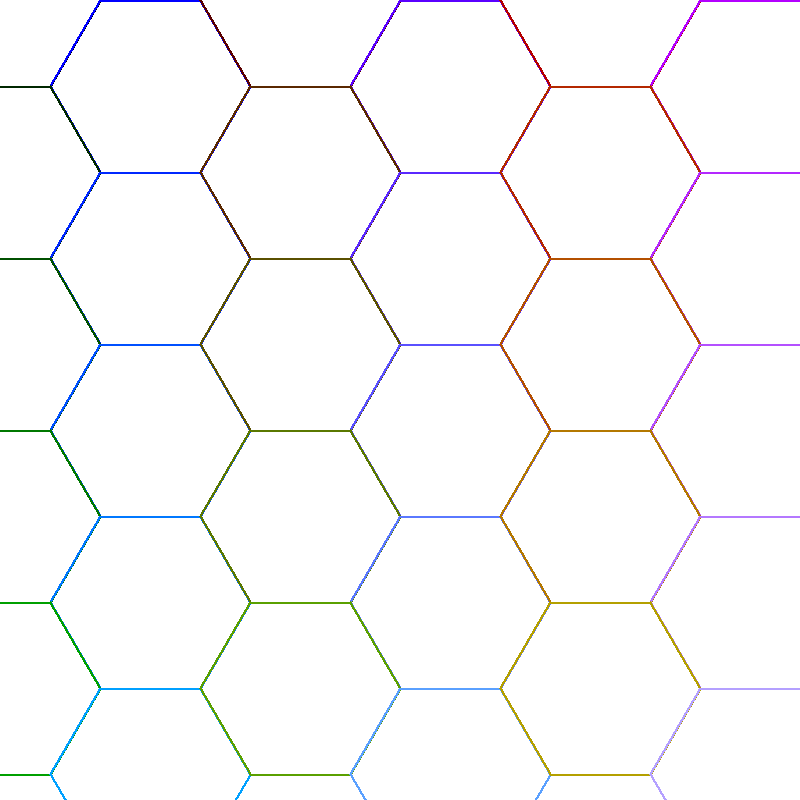
\includegraphics[width=\textwidth] {grid-hex-empty.png}
	 \caption{Empty hexagonal grid}
	 \label{fig:grid-hex-empty}
 \end{subfigure}
 \hfill
 \begin{subfigure}[b]{0.4\textwidth}
	 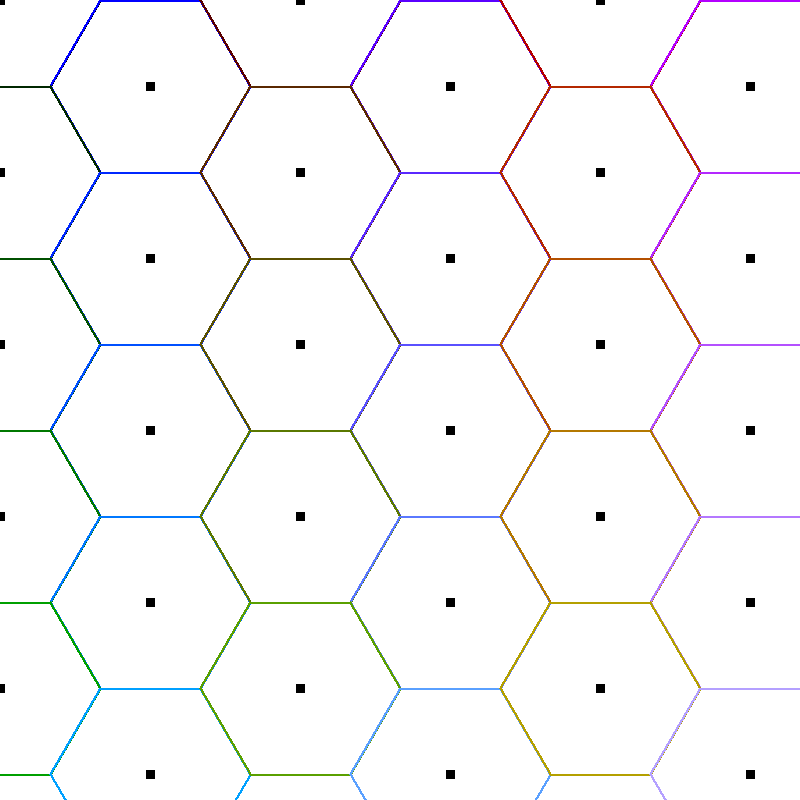
\includegraphics[width=\textwidth] {grid-hex-center.png}
	 \caption{Hexagonal grid with data at the cell centers}
	 \label{fig:grid-hex-center}
 \end{subfigure}
 \hfill
 \begin{subfigure}[b]{0.4\textwidth}
	 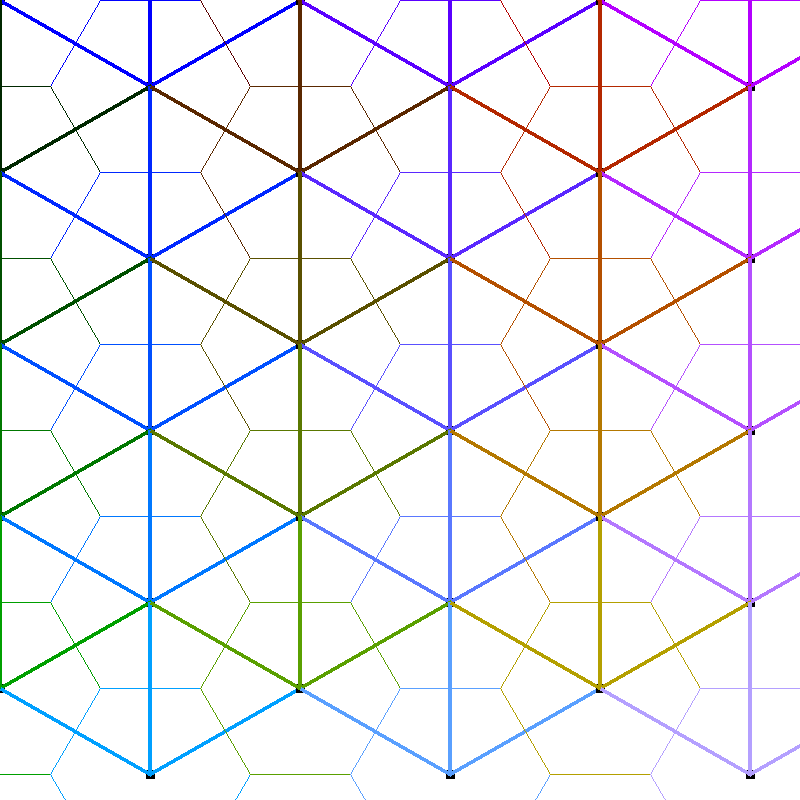
\includegraphics[width=\textwidth] {grid-hex-center_derived.png}
	 \caption{Hexagonal grid with data at the cell's centers, connected neighbours}
	 \label{fig:grid-hex-center_derived}
 \end{subfigure}
 \hfill
 \begin{subfigure}[b]{0.4\textwidth}
	 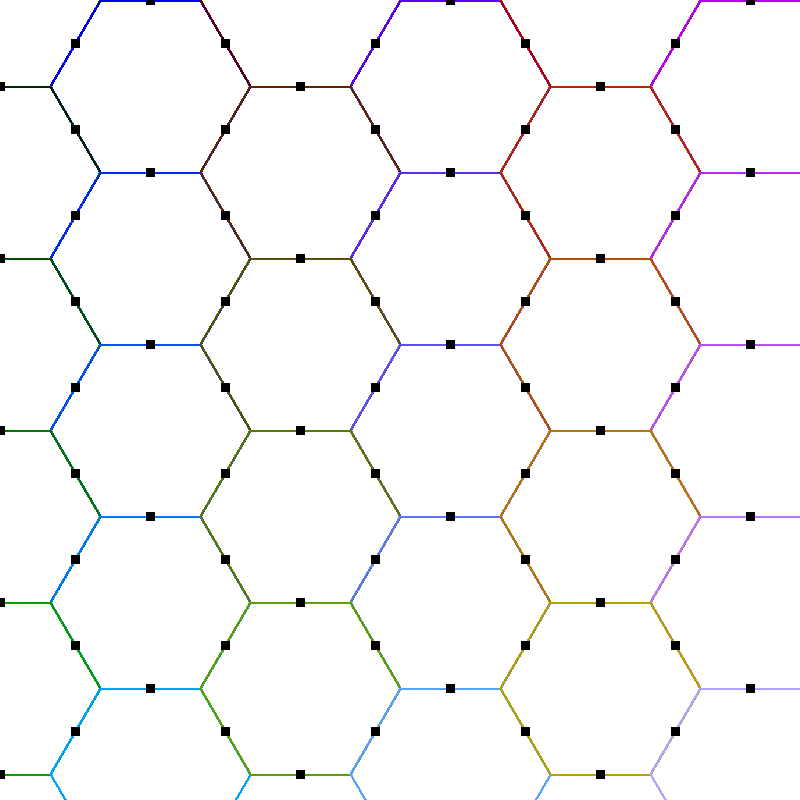
\includegraphics[width=\textwidth] {grid-hex-edges.png}
	 \caption{Hexagonal grid with data on the edges}
	 \label{fig:grid-hex-edges}
 \end{subfigure}
 \hfill
 \begin{subfigure}[b]{0.4\textwidth}
	 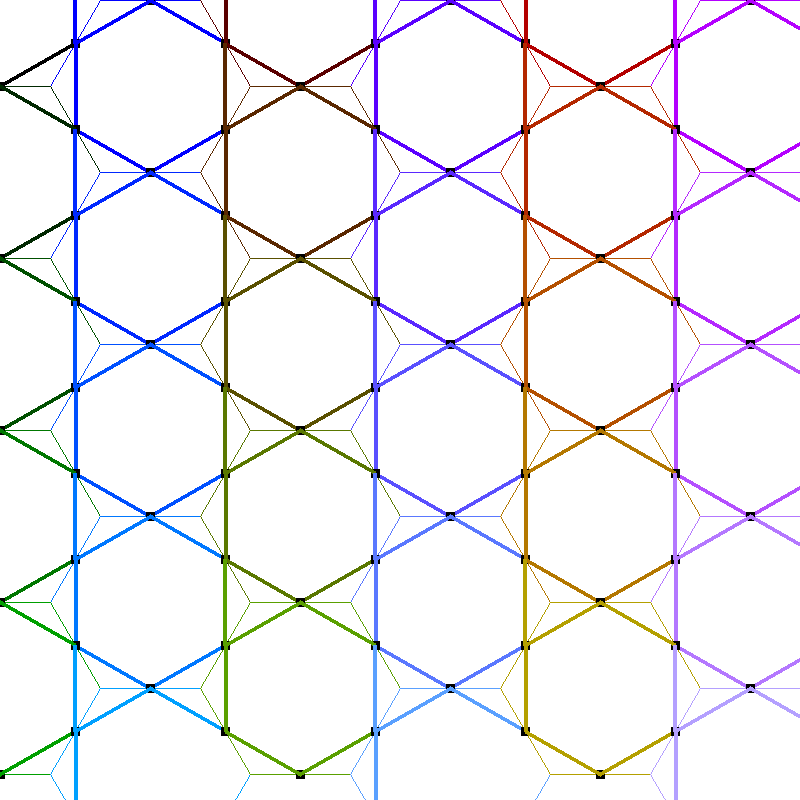
\includegraphics[width=\textwidth] {grid-hex-edges_derived.png}
	 \caption{Hexagonal grid with data on the edges, connected neighbours}
	 \label{fig:grid-hex-edges_derived}
 \end{subfigure}
 \hfill
 \begin{subfigure}[b]{0.4\textwidth}
	 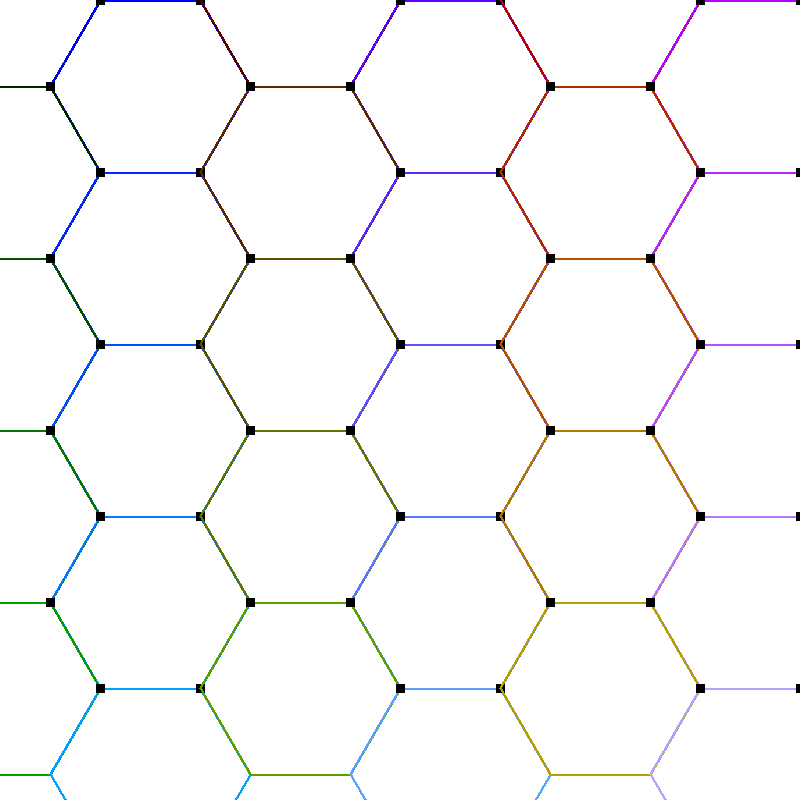
\includegraphics[width=\textwidth] {grid-hex-vertex.png}
	 \caption{Hexagonal grid with data at the vertices / connected neighbours}
	 \label{fig:grid-hex-vertex}
 \end{subfigure}

 \caption{Hexagonal grid}
 \label{fig:hexagonalgrid}
\end{figure}

\begin{figure}[!tbp]
 \centering
  \begin{subfigure}[b]{0.4\textwidth}
	 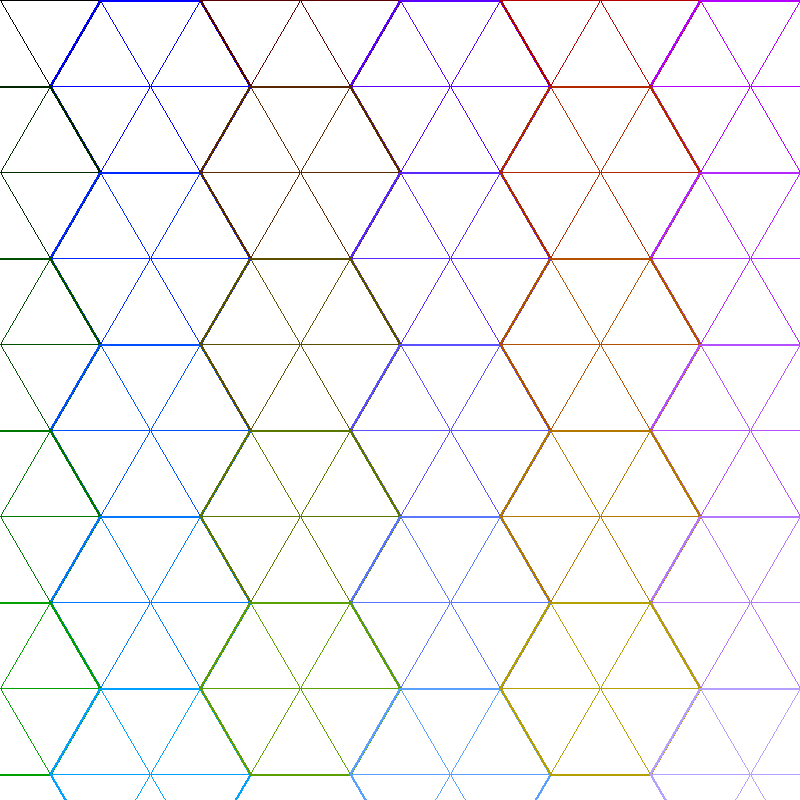
\includegraphics[width=\textwidth] {grid-triangleempty.png}
	 \caption{Empty triangular grid}
	 \label{fig:grid-triangleempty}
 \end{subfigure}
 \hfill
 \begin{subfigure}[b]{0.4\textwidth}
	 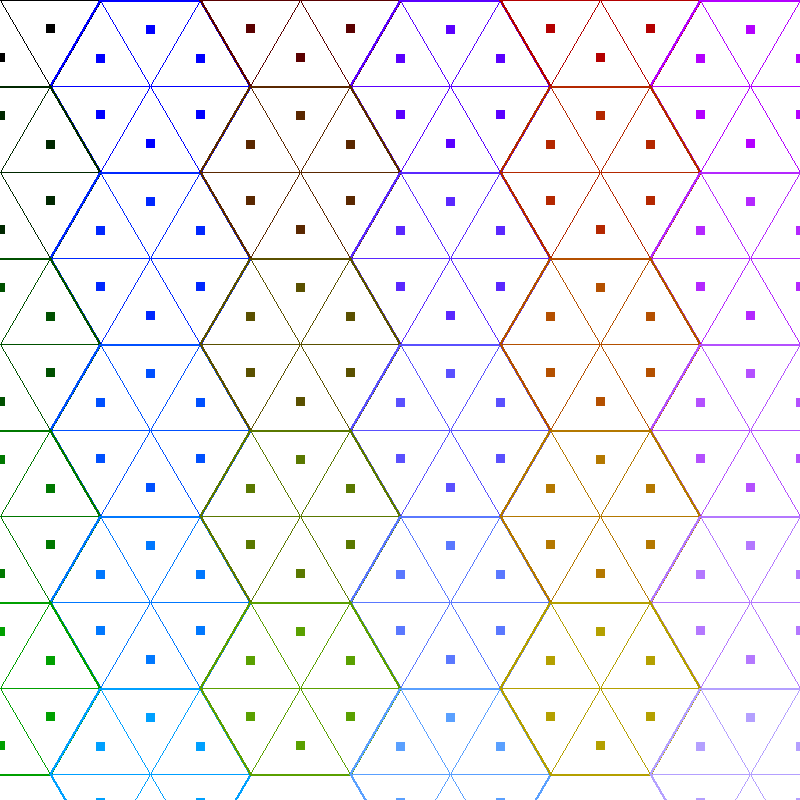
\includegraphics[width=\textwidth] {grid-trianglecenter.png}
	 \caption{Triangular grid with data at the cell centers}
	 \label{fig:grid-trianglecenter}
 \end{subfigure}
 \hfill
 \begin{subfigure}[b]{0.4\textwidth}
	 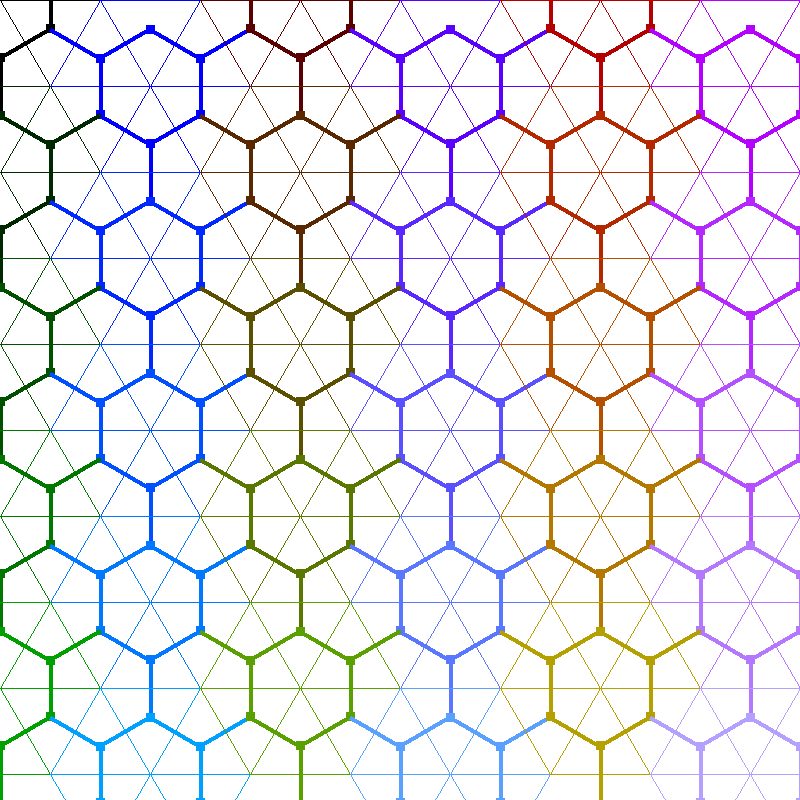
\includegraphics[width=\textwidth] {grid-trianglecenter_derived.png}
	 \caption{Triangular grid with data at the cell centers, connected neighbours}
	 \label{fig:grid-trianglecenter_derived}
 \end{subfigure}
 \hfill
 \begin{subfigure}[b]{0.4\textwidth}
	 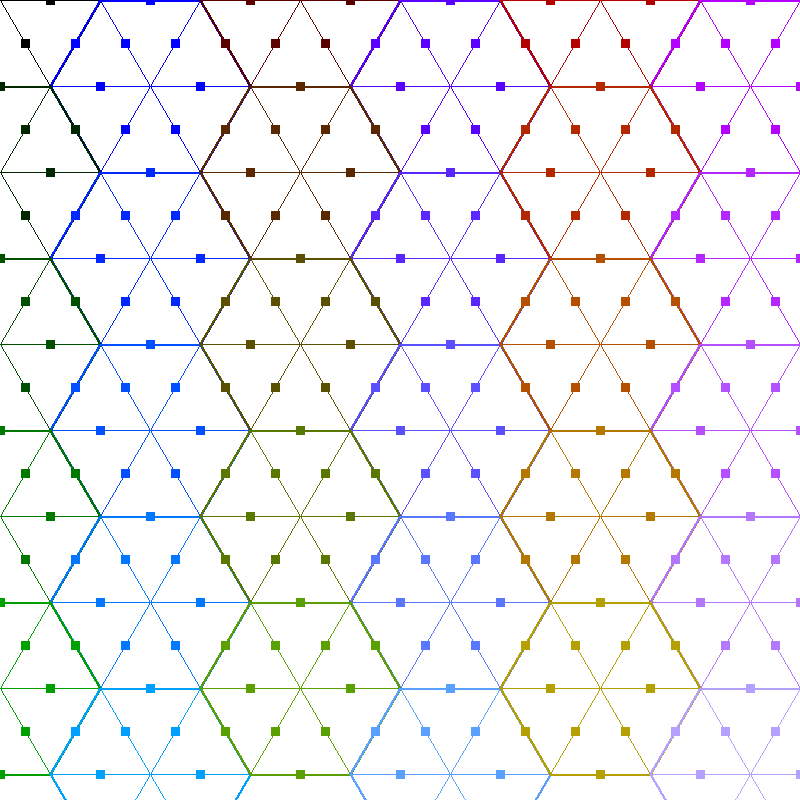
\includegraphics[width=\textwidth] {grid-triangleedges.png}
	 \caption{Triangular grid with data on the edges}
	 \label{fig:grid-triangleedges}
 \end{subfigure}
 \hfill
 \begin{subfigure}[b]{0.4\textwidth}
	 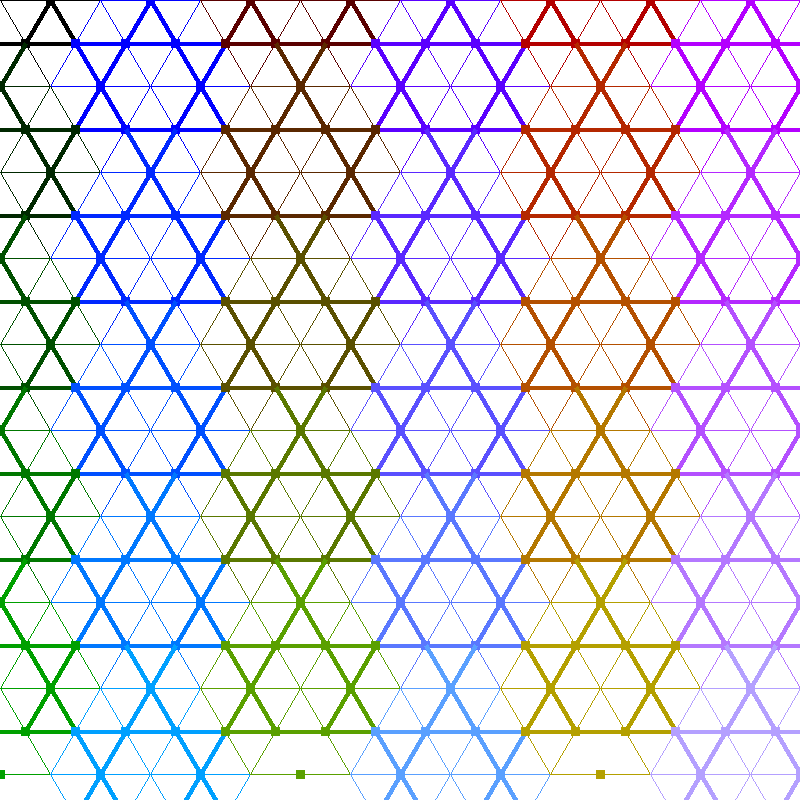
\includegraphics[width=\textwidth] {grid-triangleedges_derived.png}
	 \caption{Triangular grid with data on the edges, connected neighbours}
	 \label{fig:grid-triangleedges_derived}
 \end{subfigure}
 \hfill
 \begin{subfigure}[b]{0.4\textwidth}
	 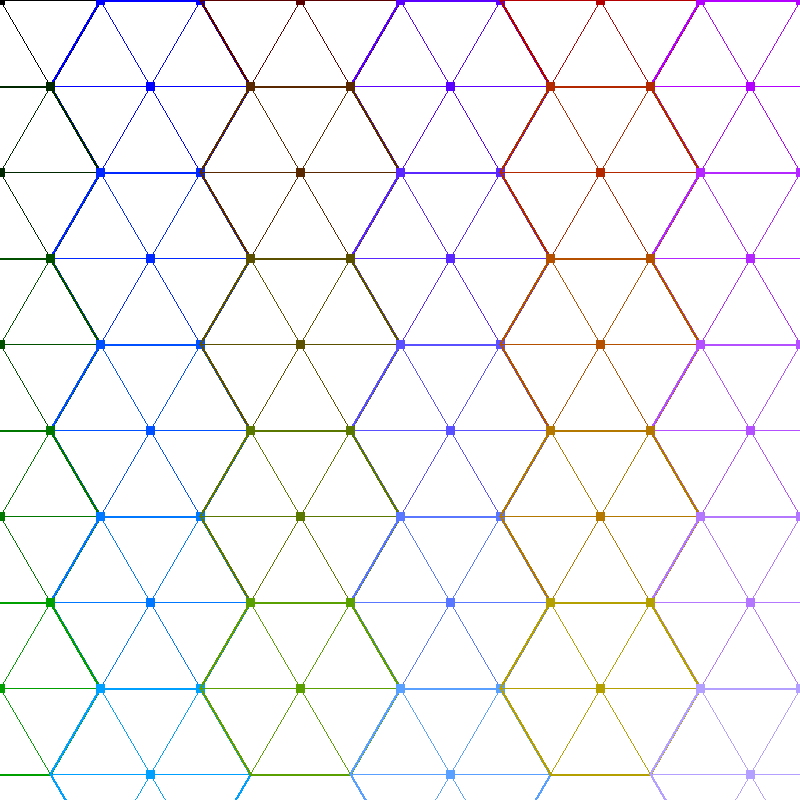
\includegraphics[width=\textwidth] {grid-trianglevertex.png}
	 \caption{Triangular grid with data on the vertices / connected neighbours}
	 \label{fig:grid-trianglevertex}
 \end{subfigure}
 \caption{Triangular grid}
 \label{fig:triangulargrid}
\end{figure}

\begin{figure}[!tbp]
 \centering
 \adjincludegraphics[trim={0 {.875\height} {.875\width} 0},clip] {test.png}
 \caption{Hilbert fitting curve}
 \label{fig:hilbert-test}
\end{figure}

\begin{figure}[!tbp]
 \centering
 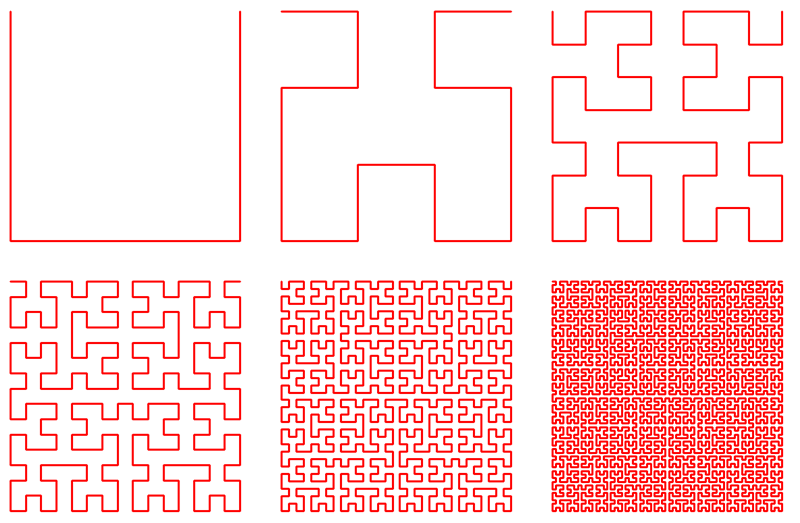
\includegraphics[width=\textwidth] {pattern.png}
 \caption{Hilbert fitting curve}
 \label{fig:hilbert-test}
\end{figure}

\paragraph{Considerations when serializing to storage systems}

\todo{JJ - What is meant here?}
When serializing a data structure to a storage system, in essence this can be done similarly than in main memory.
The address space exported by the file API of a traditional file system considers the file to be an array of bytes starting from 0.
This is quite similar to the 1D structure from main memory.
However, a general purpose language (GPL) uses variable names to point to the data in this 1D address space.
A GPL offers means to access even multi-dimensional data easily.
The user/programmer does not need to know the specific addresses in memory; addresses are calculated on within the execution environment or code of the application.
\todo{JJ - should we expand further on this? If so, I should add some diagrams... (or alternatively references)}
The main concern here is consecutive or stride access through the array; if the programmer wishes the application to loop through a given dimension of the array, memory locations would be addressed which may not be close to each other in memory, thus leading to cache misses and hence poorer performance.  The generalisation is the stride, which specifies steps through the different dimensions of the array (e.g. incrementing both dimensions of a 2D array, thus walking along the ``diagonal'').  Another special case is where the programmer needs to process the whole array, which would be done most efficiently by stepping through all the memory locations incrementally\footnote{Assuming the whole array is stored in contiguous memory, as it is in these simple examples.}, whereas looping over the dimensions and incrementing them one at a time requires more calculation and may lead to inefficient memory access with cache misses if not done correctly\footnote{Fortran historically stores 2D arrays in column-major order, whereas C and most other languages used in science store data in row-major order.}.

\todo{ problematic, as they = ?
as they are implicitly known by the code and relatively defined by the execution environment of the application in form of stack and heap.
}

When storing data from memory directly on persistent media, then the original source code is necessary to understand this data.
Similarly, the interpretation of the bytes in the data must be same when reading it back, thus, the byte order and size of the datatypes of the machine reading the data must be identical to those of the machine that wrote it.  Floating point numbers must be encoded in the same byte formats.
Since this is not always given, it threatens the longevity of our precious data, by hindering the portability and reusability of the data.

Therefore, portable data formats have been developed that allow to serialize and de-serialize data regadless of the machine's architecture.
To allow correct interpretation of a byte array, the library implementing the file format must know the data type the Bytes represent.
This information must be stored besides the actual bytes representing the data to allow later reading and interpretation.
From the user perspective, it is useful to also store further metadata describing the data.
For instance, a name and description of the contained information.
This eases not only debugging but also allows other applications to read and process data in a portable way.
File formats that contain this kind of semantical and structural metadata are called \textbf{self-describing file formats}.

Developers using a self-describing file format have to use an API to define the metadata.
Such a format may support arbitrary complex data types, which implies that some kind of data description framework must be part of the API for the file format.
See \Cref{sec: data-formats} for more information about data description frameworks.


\section{File formats}
Generally, parallel scientific applications are designed in such a way, they can solve complicated problems faster when running on a large number of compute nodes.
This is achieved by splitting a global problem into small pieces and distributing it over the compute nodes; this is called domain decomposition.
After each node has computed a local solution, they can be aggregated to one global solution.
This approach can decrease time-to-solution considerably.

I/O makes this picture more complicated, especially when data is stored in one single file and is accessed by several processes simultaneously.
In this case, problems can occur, when several processes access the same file region, e.g., two processes can overwrite the data of each other, or inconsistencies can occur when one process reads, while another writes.
Portability is another issue: When transferring data from one platform to another, the contained information should still be accessible and identical.
The purpose of I/O libraries is to hide the complexity from scientists, allowing them to concentrate on their research.



\begin{table}
  \centering
  \begin{tabular}{l|l|l|l}
    Name      & Fullname                   & Version & Developer \\
    \hline
    GRIB1     & GRIdded Binary             & 1       & World Meteorological Organization\\
    GRIB2     & GRIdded Binary             & 2       & World Meteorological Organization\\
    NetCDF3   & Network Common Data Form   & 3.x     & Unidata (UCAR/NCAR)\\
    NetCDF4   & Network Common Data Format & 4.x     & Unidata (UCAR/NCAR\\
    HDF4      & Hierarchical Data Format   & 4.x     & NCSA/NASA\\
    HDF4-EOS2 & HDF4-Earth Obseving System & 2       & \\
    HDF5      & Hierarchical Data Format   & 5.x     & NCSA/NASA\\
    HDF5-EOS5 & HDF5-Earth Obseving System & 5       & \\
\end{tabular}
\caption{Parallel data formats}
\label{tab:fformats}
\end{table}


Some common file formats are listed in the \Cref{tab:fformats}.
All of these formats are portable (machine independent) and self-describing.  
Self-describing means, that files can be examined and read by the appropriate software without the knowledge about the structural details of the file.  
The files may include additional information about the data, called ``metadata''.
Often, it is textual information about each variable's contents and units (e.g.,"humidity" and "g/kg") or numerical information describing the coordinates (e.g., time, level, latitude, longitude) that apply to the variables in the file.

GRIB is a record format, NetCDF/HDF/HDF-EOS formats are file formats.
%It is the difference.
In contrast to record format, file formats are bound to format specific rules.
For example, all variable names in NetCDF must be unique.
In HDF, although, variables with the same name are allowed, they must have different paths.
No such rules exist for GRIB.
It is just a collection of records (datasets), which can be appended to the file in any order. 

GRIB-1 record (aka, 'message') contains information about two horizontal dimensions (e.g., latitude and longitude) for one time and one level. 
GRIB-2 allows each record to contain multiple grids and levels for each time. 
However, there are no rules dictating the order of the collection of GRIB records (e.g, records can be in random chronological order).

\todo{relate to chapter 4?  "data description frameworks"}

%Not HPC:
Finally, a file format without parallel I/O support, but still worth to mention, is CSV (comma-separated values).
It is special due to its simplicity, broad acceptance and support by a wide range of applications.
The data is stored as plain text in a table. 
Each line of the file is a data record. 
Each record consists of one or more fields, that are separated by commas (hence the name).
The CSV file format is not standardized.
There are many implementations that support additional features, e.g., other separators and column names.



\subsection{NetCDF4}
NetCDF4 with Climate Forecast (CF) metadata and GRIB evolved to the de-facto standard formats for  convenient data access for the scientists in the domain of NWP and climate.
For convenient data access, it provides a set of features, for example, metadata can be used to assign names to variables, set units of measure, label dimensions, and provide other useful information.
The portability allows data movement between different possibly incompatible platforms, which simplifies the exchange of data and facilitates communication between scientists.
The ability to grow and shrink datasets, add new datasets and access small data ranges within datasets simplifies the handling of data a lot.
%HPC: Sharable
The shared file allows to keep the data in same file.
Unfortunately, the last feature conflicts with performance and efficient usage of the state-of-art HPC.
The files, which are accessed simultaneously by several processes, cause a lot of synchronisation overhead which slows down the I/O performance.
Synchronization is necessary to keep the data consistent.
%Performance: Compression, Chunking

% Relation between HPC imbalance and compression 
The rapid development of computational power and storage capacity, and slow development of network bandwidth and I/O performance in the last years resulted in imbalanced HPC systems.
The application use the increased computational power to process more data.
More data, in turn, requires more costly storage space, higher network bandwidth and sufficient I/O performance on storage nodes.
But due to imbalance, the network and I/O performance are the main bottlenecks.
The idea is, to use a part of the computational power for compression, adding a little extra latency for the transformation while significantly reducing the amount of data that needs to be transmitted or stored.

% Transition to NetCDF4 and HDF5
Before considering a compression method for HPC, it is a good idea to take a look at the realization of parallel I/O in modern scientific applications.
Many of them use the NetCDF4 file format, which, in turn, uses HDF5 under the hood.
 
\subsection{Typical NetCDF Data Mapping}
\label{sec:netcdfDataMapping}
\Cref{lst:NetCDF-data} gives an example for scientific metadata stored in a NetCDF file.
Firstly, between Line 1 and 4, a few dimensions of the multidimensional data are defined.
Here there are longitude, latitude with a fixed size and time with a variable size that allows to be extended (appending from a model).
Then different variables are defined on one or multiple of the dimensions.
The longitude variable provides a measure in “degreees east” and is indexed with the longitude dimension; in that case the variable longitude is an 1D array that contains values for an index between 0-479. 
It is allowed to define attributes on variables, this scientific metadata can define the semantics of the data and provide information about the data provenance.
In our example, the unit for longitude is defined in Line\,7.
Multidimensional variables such as \texttt{sund} (Line 45) are defined on an 2D array of values for the longitude and latitude over various timesteps.
The numeric values contain a scale factor and offset that has to be applied when accessing the data; since the data is here stored as short values, it should be converted to floating point data in the application.
The \texttt{\_FillValue} indicates a default value for missing data points.

Finally, global attributes such as indicated in Line\,54\,ff. describe that this file is written with the NetCDF-CF schema and its history describes how the data has been derived / extracted from original data.

\begin{tcbcode}[label={lst:NetCDF-data}]{Example NetCDF metadata}
\begin{lstlisting}
dimensions:
	longitude = 480 ;
	latitude = 241 ;
	time = UNLIMITED ; // (1096 currently)
variables:
	float longitude(longitude) ;
		longitude:units = "degrees_east" ;
		longitude:long_name = "longitude" ;
	float latitude(latitude) ;
		latitude:units = "degrees_north" ;
		latitude:long_name = "latitude" ;
	int time(time) ;
		time:units = "hours since 1900-01-01 00:00:0.0" ;
		time:long_name = "time" ;
		time:calendar = "gregorian" ;

	short t2m(time, latitude, longitude) ;
		t2m:scale_factor = 0.00203513170666401 ;
		t2m:add_offset = 257.975148205631 ;
		t2m:_FillValue = -32767s ;
		t2m:missing_value = -32767s ;
		t2m:units = "K" ;
		t2m:long_name = "2 metre temperature" ;
	short sund(time, latitude, longitude) ;
		sund:scale_factor = 0.659209863732776 ;
		sund:add_offset = 21599.6703950681 ;
		sund:_FillValue = -32767s ;
		sund:missing_value = -32767s ;
		sund:units = "s" ;
		sund:long_name = "Sunshine duration" ;

// global attributes:
		:Conventions = "CF-1.0" ;
		:history = "2015-06-03 08:02:17 GMT by grib_to_netcdf-1.13.1: grib_to_netcdf /data/data04/scratch/netcdf-atls14-a562cefde8a29a7288fa0b8b7f9413f7-lFD4z9.target -o /data/data04/scratch/netcdf-atls14-a562cefde8a29a7288fa0b8b7f9413f7-CyGl1B.nc -utime" ;
}
\end{lstlisting}
\end{tcbcode}



\newpage
\section{Typical Workflows}

\subsection{NWP}




\todo{UC: ask for DWD Weather use cases; ....}


\subsubsection{WUC1: Incoming Stream of Observations}

satellites
radar
weather stations
ships

\subsubsection{WUC2: Pre-Processing}

insufficient sampling makes preprocessing necessary so models can be intialised correctly


\subsubsection{WUC3: Now Casting (0-6h)}

directly inffered from satellite data and weather stations

most importantly extrapolation of radar echos

usually for warnings




\subsubsection{WUC4: Numeric Model Forecasts (0-10+ Days)}

\begin{enumerate}
	\item Read-Phase to intialise simulation
	\item periodic snapshots (write) for time evolution
\end{enumerate}


\subsubsection{WUC5: Post-Processing}

nowcasting:
multi sensor integration
classification
ensembles
impact models

model:
statistical interpretation
model-combination



generation of GRIB files as services to customers of weather forecasts


\subsubsection{WUC6: Visualisation}

of many variables available in a simulation only a view are read and visualised

timeseries




\subsection{Characteristics of Workload Mix}

The systems are shared so it is distinguished between emergent system behaviour and workload of individual applications.

How are the shares for different workloads on the system?

e.g. 10\% of applications are CUC1, 20\% WUC1, ...


We assume that in principle this mix changes over time, but a specialized data centre makes only sense as long some things are somewhat stable...


\todo{Discuss with DKRZ/App team, there should be a paper or something as the workload mix is also considered for procurements}

E.g. DKRZ...regular load at every point in time is about 20 GByte/s 








\subsection{Climate}

\subsubsection{CUC1: Writing Data from a Parallel Program}

We have P processes utilizing PPN cores per node.
Iterative program.
Asynchronous communication and I/O ?
Every I iterations, a subset of memory capacity $C_I$ should be persisted.
After T iterations, the program terminates and writes $C_T$ capacity for a snapshot.
This process may be repeated, restarting from a snapshot to simulate 100 or 1000 of years of climate.

What people do right now:
- store AND Keep every checkpoint, may be used for later analysis and for re-computation.
- Some people only keep every 10th of a checkpoint (as the costs to recompute 9 other checkpoints is less than storing 10).




ICON
	I/O coordinators, write out groups of variables..
	variables at different intervals
	individual variables are not yet parallel




%%%%%%%%%%%%%%%%%%%%%%%%%%%%%%%%%%%%%%%%%%%%%%%%%%%%%%%%%%%%%%%%%%%%%%%%%%%%%%%
\subsubsection{CUC2: Post-Processing Data}

A scientist reads a time series produces from multiple runs of the parallel program (see \ref{TODO}).
He/she may want to read a subset of data points (i.e., an area of interest) across all time steps.





%%%%%%%%%%%%%%%%%%%%%%%%%%%%%%%%%%%%%%%%%%%%%%%%%%%%%%%%%%%%%%%%%%%%%%%%%%%%%%%
\subsubsection{CUC3: Post-Processing: Partial CDO}

\todo{What kind of user behaivor is common? Is the same user, applying the same CDO to many many records?}





%%%%%%%%%%%%%%%%%%%%%%%%%%%%%%%%%%%%%%%%%%%%%%%%%%%%%%%%%%%%%%%%%%%%%%%%%%%%%%%
\subsubsection{CUC4: Visualisation}

\todo{are the challenges for climate visualisation different from weather?}


vtk
paraview


of many variables available in a simulation only a view are read and visualised

timeseries
average e..g temperature anomaly

expensive cloud visualisation..





%%%%%%%%%%%%%%%%%%%%%%%%%%%%%%%%%%%%%%%%%%%%%%%%%%%%%%%%%%%%%%%%%%%%%%%%%%%%%%%
\section{Use cases from a data access perspective}

\todo{JL: Decide where this fits best.}








%%%%%%%%%%%%%%%%%%%%%%%%%%%%%%%%%%%%%%%%%%%%%%%%%%%%%%%%%%%%%%%%%%%%%%%%%%%%%%%
\chapter{Background and Related Work}

\begin{chapterIntro}
This chapter gives an overview to related work in the area of I/O research for HPC and Big Data.
Then, alternative approaches for defining data structures within scientific middleware are introduced.
\end{chapterIntro}


\section{Exascale I/O}

%Fast Forward

%DARPA ExaScale Computing Study


%DOE Storage?


%Exa HDF5	
%	!!


%HDF5 VOL
%burst buffers
%fastforward HDF5


%\cite{darpa_exascale_2011} indentifies four major areas with challenges on the way to achieving exascale systems: Energy and Power, Memory and Storage, Concurrency and Locality, Resilience.

%In regard to storage the report 

% Cited from Darpa:
% \begin{quote}
% The Memory and Storage Challenge concerns the lack of currently available technology
% to retain data at high enough capacities, and access it at high enough rates, to support the
% desired application suites at the desired computational rate, and still fit within an acceptable
% power envelope. This information storage challenge lies in both main memory (DRAM today)
% and in secondary storage (rotating disks today).
% \end{quote}


% Cited from DARPA on Concurrency and Locality:
% \begin{quote}
% The Concurrency and Locality Challenge likewise grows out of the flattening of silicon
% clock rates and the end of increasing single thread performance, which has left explicit, largely
% programmer visible, parallelism as the only mechanism in silicon to increase overall system
% performance. While this affects all three classes of systems, projections for the data center
% class systems in particular indicate that applications may 
%%%%%%%%%%%%%%%%%%%%%%%%%%%%%%%%%%%%%%%%%%%%%%%%%%%%%%%%%%%%%%%have to support upwards of a billion
% separate threads to efficiently use the hardware.
% \end{quote}




%Due to the increasing workloads' complexity in modern HPC clusters, which nowadays include generation, analysis and sharing of data among multiple sites, several projects have explored the benefit of using these new features. %some of the aforementioned libraries have evolved to support more flexible data management mechanisms. 
%Along this line, 
The advent of exascale computing is exacerbating the gap between computational performance (measured in FLOPS) and the capability of the storage system to feed data into the computational pipelines at a sufficient speed (measured in GB/s). Indeed, today's storage infrastructures still heavily rely on spinning disk drives, which performance have not scaled at the same pace of the compute components. Along with the computing power also grows the amount of data that can be generated/analysed, and thus the size of the corresponding datasets in the storage system. This aspect also affects the complexity of scientific workflows that nowadays need to account for the generation (simulation codes or sensor), analysis (extraction of meaningful information), and finally sharing of large datasets with the research community. All these requirements have been driving many different research projects and efforts to build efficient I/O libraries. Weather and Climate communities have used some of these libraries for years and have also relied on them to decouple data view at the application level (multidimensional arrays) from data representation in the storage backend (one dimensional array). NetCDF~\cite{netcdf} and GRIB~\cite{grib} are the I/O libraries of choice for the Climate and Weather communities respectively. The NetCDF library relies on additional I/O service libraries to work. In particular NetCDF4 exploits the HDF5~\cite{hdf5} library to organise as well as to read/write data from/to the file system. We will explore some ESDM relevant aspects of these libraries in the rest of this section. The HDF5 library is modular and allows for different implementations of the I/O transfer mechanism, as well as for different I/O optimisations. 

The Distributed Shared Memory driver, HDF5dsm~\cite{soumagne:hal-00652816}, takes advantage of the HDF5 modularity in the Virtual File Layer (VFL) to transparently redirect data from disks to staging nodes that will later use this data for post processing analysis, thus making the building of computing pipelines simpler and more efficient (reduced total time to solution). On the same line the Adaptable I/O System, ADIOS~\cite{Liu:2014:HAC:2768261.2768267}, provides an interface independent I/O middleware in which specific I/O transports (e.g. HDF5, NetCDF, POSIX) and optimisations (N-1, N-M, N-N) are encoded in a separate XML file. The ADIOS code at the application level remains fairly simple, just declaring what variables should be written and how big they are. All the details about how these variables are effectively transfered are hidden in the XML file, making the middleware adaptable. Similarly to HDF5dsm, ADIOS provides mechanisms to stage data in apposite nodes for later indexing construction, compression, and/or post processing. Unlike the HDF5dsm driver, which uses the same familiar HDF5 API at the user level, ADIOS requires modifications of the application source, making its adoption in legacy codes not feasible. Besides data staging and indexing the library also supports data provenance and advanced techniques for data mining to drive, e.g., effective pre-fetching. Nevertheless, the ADIOS library still relies on the legacy POSIX-IO interface and does not give the user the flexibility to distribute his data to different backends according to data characteristics.

The Fast Forward I/O project~\cite{intel_fast_2014}, from the U.S. Department of Energy (DOE), has built an Exascale ready storage infrastructure called Distributed Application Object Storage (or DAOS) based on a Lustre file system with object storage extensions (as the storage backend) and the HDF5 library as the data format interface for manipulating/storing/retrieving data. In this context, the HDF5 library has been extended with a Virtual Object Layer (VOL) to support the new object storage capabilities offered by the extended Lustre~\cite{hdfgroup_future_2015} and to support new NVM technologies to burst buffer data at intermediate nodes (Burst Buffer I/O Nodes) before writing it to Lustre. Additionally, a VOL plug-in for the Parallel Log-structured File System (PLFS) has been developed to allow HDF5 to store data on PLFS~\cite{Bent:2009:PCF:1654059.1654081} using alternative mappings~\cite{mehta_plugin_2012}.
Dong et al~\cite{dong_expediting_2013} have used the HDF5 VOL to build the Scientific Data Service (SDS) framework, adapting the layout of stored data to the specific I/O pattern of applications retrieving it. Similarly to Fast Forward I/O the EC funded SAGE (percipient StorAGe for Exascale data centric computing)~\cite{sage} project aims at building a Big Data Extreme Computing (BDEC) storage infrastructure based on the Mero object store~\cite{sage-wp} and new 3D-Xpoint memory technology. One of the most interesting features of the SAGE system is the ability to offload parts of the computation to the storage nodes and retrieve the results of the computation afterwards, thus minimising data movement and energy consumption. The SAGE project is also exploring advanced analytics techniques on the storage system performance metadata, opening the possibility for automatic tuning of the storage parameters.

The Dynamic Exascale Entry Platform Extended Reach (DEEP-ER) project is building an extreme scale platform based on the BeeGFS file system and the integration of NVM and Network Attached Memory (NAM) technologies in the storage hierarchy~\cite{deep-er}. In DEEP-ER exascale level fault tolerance is achieved by combining the Scalable Checkpoint Restart (SCR)~\cite{Moody:2010:DME:1884643.1884666} buddy checkpointing capabilities withe the SIONlib library, which takes care of storing the checkpoint data using a unified file format. At the data format library level the HDF group is also working on the ExaHDF5 project to provide efficient parallel I/O handling for the movement of massive amounts of data and extending the HDF5 API with a query API that can be used by other tools to selectively extract information from datasets~\cite{exahdf5}.

All the works mentioned so far solve some of the well known I/O pain points typically found when moving to extreme scale. Nevertheless, none of these works has addressed the problem of format independent data access. Every I/O library can only access data that has been stored using that particular format and cannot, on the other hand, understand the format of other libraries. This makes the use of data in scientific workflows cumbersome, since data may need to be stored in one format and then transformed to be fed to the next stage of processing (e.g. store a dataset into a HDFS file system to be processed by a Hadoop cluster). Sharing also becomes very complex since data has to be converted to the target format before it can be used, causing a waste of compute and storage resources. The ESD middleware addresses this problem and takes advantage of the lessons learned by other projects to optimise I/O performance at the same time.
%The proposed ESD middleware extends these use cases to support a wider range of use cases, scientific libraries and hardware configurations.
%\cite{bader_accelerated_2014} ACME on 


%%%%%%%%%%%%%%%%%%%%%%%%%%%%%%%%%%%%%%%%%%%%%%%%%%%%%%%%%%%%%%%%%%%%%%%%%%%%%%%
%section{Big Data Storage}
%n the context of Big Data, there are many (typically Java based) technologies that address storing and processing of large quantities of data.
%
%he Hadoop File System (HDFS) is a distributed file system that is designed to work with 
%ommodity hardware\cite{shvachko2010hadoop}.
%t provides fault tolerance via data replication and self healing.
%ne limitation of its design is its consistency semantics which allows concurrent reads of multiple processes but only a single writer.
%ts suboptimal performance on high-performance storage and assumption to work on cheap hardware makes it no optimal choice for HPC environments.
%herefore, many vendors support HDFS adapters on top of high-performance parallel file systems such as GPFS and Lustre.
%
%ive\cite{thusoo2010hive} utilizes data stored on HDFS and other Big Data solutions and
%ffers a convenient SQL interface to this data.
%his allows users to explore data using SQL by accessing data stored on the file system.
%he advantage is that no extract, transform, load (ETL) process is necessary;
%imply move the data into the file system, create a scheme on the existing files.
%
%rill \footnote{\url{https://drill.apache.org}} also provides an SQL interface to existing data.
%imilar to Hive existing data can be adjusted, but in the case of Drill, data may be stored on various storage backends such as simple JSON file, on Amazon S3, or MongoDB.
%
%ciSpark\footnote{\url{https://github.com/SciSpark/SciSpark}} is an extension to the Spark data processing engine that allows to access scientific file formats such as NetCDF from Spark programs.
%herewith, the costs for data conversion is omitted.
%
%lluxio \footnote{\url{https://www.alluxio.com/docs/community/1.3/en/}} offers a scalable in-memory file system.
%n interesting feature is that one can attach (mount) data from multiple (even remote) endpoints such as S3 into the hierarchical in-memory namespace.
%t provides control to the in-memory data, for example, to trigger a flush of dirty data to the storage backend and an interface for pinning data in memory (similar to burst buffer functionality).
%ata stored on Alluxio can be used on various big data tools. 
%
%todo{Add notes about edgent and avro}
%
%comment{
%ttp://edgent.incubator.apache.org/
%pache Edgent is a programming model and micro-kernel style runtime that can be embedded in gateways and small footprint edge devices enabling local, real-time, analytics on the continuous streams of data coming from equipment, vehicles, systems, appliances, devices and sensors of all kinds (for example, Raspberry Pis or smart phones). Working in conjunction with centralized analytic systems, Apache Edgent provides efficient and timely analytics across the whole IoT ecosystem: from the center to the edge.
%dgent is an open source programming model and runtime for edge devices that enables you to analyze streaming data on your edge devices. When you analyze on the edge, you can:
%   Reduce the amount of data that you transmit to your analytics server
%   Reduce the amount of data that you store
%ava source code...
%ou can send data from an Apache Edgent application to your back-end system when you need to perform analysis that cannot be performed on the edge device....
%
%
%ttp://avro.apache.org/docs/current/spec.html
%ttps://avro.apache.org/docs/1.8.0/api/cpp/html/index.html
%ntroduction to Avro C++
%vro is a data serialization system. See http://avro.apache.org/docs/current/ for background information.
%vro C++ is a C++ library which implementats parts of the Avro Specification. The library includes the following functionality:
%
%
%%%%%%%%%%%%%%%%%%%%%%%%%%%%%%%%%%%%%%%%%%%%%%%%%%%%%%%%%%%%%%%%%%%%%%%%%%%%%%%
%subsection{MongoDB}
%he MongoDB\footnote{\url{https://docs.mongodb.com/}} is an open-source document database.
%ts architecture is high-performant and horizontally scalable for clusters systems.
%ongoDB offers a rich set of interface, e.g., RESTful access, C, Python, Java.
%
%he data model of MongoDB provides three levels:
%begin{itemize}
% \item Database: follows our typical notion; permissions are defined on the database level.
% \item Document: This is a BSON object (binary JSON) -- consisting of subdocuments with data.
% An example as JSON is shown in \Cref{lst:mongoJSON}.
% Each document has the primary key field: \_id. The field must be either manually set or it will be automatically filled.
% 
% \item Collection: this is like a table of documents in a database. Documents can have individual schemas. It supports indexes on fields (and compound fields).
%end{itemize}
%o access data, one has to know the name of a database (potentially secured with a username and password), collection name. All documents within the collection can be searched or manipulated with one operation. 
%
%n the example of \Cref{lst:mongoJSON}, it would also been possible to create one document for each person and use the $_id$ field with a self-defined unique ID such as a tax number.
%
%begin{tcbcode}[label={lst:mongoJSON}]{Example MongoDB JSON document}
%begin{lstlisting}
%_id" : ObjectId("43459bc2341bc14b1b41b124"),
%people" : [ # subdocuments:
%   { "name" : "Max", "id" : 4711, "birth" : ISODate("2000-10-01")},
%   { "name" : "Lena", "id" : 4712, "birth", ... }  
% ] 
%end{lstlisting}
%end{tcbcode}
%
%
%ongoDB's architecture uses sharding of document keys to partition data across different servers.
%ervers can be grouped into replica sets to provide high availability and fault tolerance.
%
%paragraph{Query documents}
%
% query document is a BSON document that is used to search all documents of a collection for data that matches the defined query.
%he example in \Cref{lst:mongoQuery} specifies documents that contain the subdocument people with an id field that is bigger than 4711.
%omplex queries can be defined.
%n combination with indexes on fields, MongoDB can search large quantities of documents quickly.
%
%begin{tcbcode}[label={lst:mongoQuery}]{Example MongoDB Query document}
%begin{lstlisting}
% "people.id" : { $gt : 4711 } }
%end{lstlisting}
%end{tcbcode}
%

%%%%%%%%%%%%%%%%%%%%%%%%%%%%%%%%%%%%%%%%%%%%%%%%%%%%%%%%%%%%%%%%%%%%%%%%%%%%%%%
\section{Data Description Frameworks} \label{sec: data-formats}
Many application developers rely on data description frameworks or libraries to manage datatypes\footnote{A datatype is a collection of properties, all of which can be stored on storage and which, when taken as a whole, provide complete information for data conversion to or from the datatype.}. Different libraries and middlewares provide mechanisms to describe data using basic types and to construct new ones using dedicated APIs. Datatypes are provided as a transparent conversion mechanism between internal representation (as data is represented in memory) and external representation (how data is transmitted over the network or saved to permanent storage). This section gives an overview of datatypes provided by different software packages. 
Starting from existing middlewares' datatype definitions, we will propose a list of basic datatypes to be supported by the ESD middleware.

%The benefits are manifold and many different projects are available.

%%%%%%%%%%%%%%%%%%%%%%%%%%%%%%%%%%%%%%%%%%%%%%%%%%%%%%%%%%%%%%%%%%%%%%%%%%%%%%%
\subsection{MPI}
The Message Passing Interface supports derived datatypes for efficient data transfer as well as compact description of file layouts (through file views). MPI defines a set of basic datatypes (or type class) from which more complex ones can be derived using appropriate data constructor APIs. Basic datatypes in MPI resemble C atomic types as shown in \Cref{table: mpi-types}.

\begin{longtable}{|>{\centering\arraybackslash} m{5.5cm} | >{\centering\arraybackslash} m{6cm} |}\hline\hline
        \cellHeader Datatype                  & \cellHeader Description                                                               \\ \hline
        \small \texttt{MPI\_CHAR}                     & \small this is the traditional ASCII character that is numbered by integers between 0 and 127 \\ \hline
        \small \texttt{MPI\_WCHAR}                    & \small this is a wide character, e.g., a 16-bit character such as a Chinese ideogram          \\ \hline
        \small \texttt{MPI\_SHORT}                    & \small this is a 16-bit integer between -32,768 and 32,767                                    \\ \hline
        \small \texttt{MPI\_INT}                      & \small this is a 32-bit integer between -2,147,483,648 and 2,147,483,647                      \\ \hline
        \small \texttt{MPI\_LONG}                     & \small this is the same as MPI\_INT on IA32                                                   \\ \hline
        \small \texttt{MPI\_LONG\_LONG\_INT}          & \small this is a 64-bit long signed integer, i.e., %
                                                        an integer number between -9,223,372,036,854,775,808 and 9,223,372,036,854,775,807            \\ \hline
        \small \texttt{MPI\_LONG\_LONG}               & \small same as MPI\_LONG\_LONG\_INT                                                           \\ \hline
        \small \texttt{MPI\_SIGNED\_CHAR}             & \small same as MPI\_CHAR                                                                      \\ \hline
        \small \texttt{MPI\_UNSIGNED\_CHAR}           & \small this is the extended character numbered by integers between 0 and 255                  \\ \hline
        \small \texttt{MPI\_UNSIGNED\_SHORT}          & \small this is a 16-bit positive integer between 0 and 65,535                                 \\ \hline
        \small \texttt{MPI\_UNSIGNED\_LONG}           & \small this is the same as MPI\_UNSIGNED on IA32                                              \\ \hline
        \small \texttt{MPI\_UNSIGNED}                 & \small this is a 32-bit unsigned integer, i.e., a number between 0 and 4,294,967,295          \\ \hline
        \small \texttt{MPI\_FLOAT}                    & \small this is a single precision, 32-bit long floating point number                          \\ \hline
        \small \texttt{MPI\_DOUBLE}                   & \small this is a double precision, 64-bit long floating point number                          \\ \hline
        \small \texttt{MPI\_LONG\_DOUBLE}             & \small this is a quadruple precision, 128-bit long floating point number                      \\ \hline
        \small \texttt{MPI\_C\_COMPLEX}               & \small this is a complex float                                                                \\ \hline
        \small \texttt{MPI\_C\_FLOAT\_COMPLEX}        & \small same as MPI\_C\_COMPLEX                                                                \\ \hline
        \small \texttt{MPI\_C\_DOUBLE\_COMPLEX}       & \small this is a complex double                                                               \\ \hline
        \small \texttt{MPI\_C\_LONG\_DOUBLE\_COMPLEX} & \small this is a long double complex                                                          \\ \hline
        \small \texttt{MPI\_C\_BOOL}                  & \small this is a \_Bool                                                                       \\ \hline
        \small \texttt{MPI\_INT8\_T}                  & \small this is a 8-bit integer                                                                \\ \hline
        \small \texttt{MPI\_INT16\_T}                 & \small this is a 16-bit integer                                                               \\ \hline
        \small \texttt{MPI\_INT32\_T}                 & \small this is a 32-bit integer                                                               \\ \hline
        \small \texttt{MPI\_INT64\_T}                 & \small this is a 64-bit integer                                                               \\ \hline
        \small \texttt{MPI\_UINT8\_T}                 & \small this is a 8-bit unsigned integer                                                       \\ \hline
        \small \texttt{MPI\_UINT16\_T}                & \small this is a 16-bit unsigned integer                                                      \\ \hline
        \small \texttt{MPI\_UINT32\_T}                & \small this is a 32-bit unsigned integer                                                      \\ \hline
        \small \texttt{MPI\_UINT64\_T}                & \small this is a 64-bit unsigned integer                                                      \\ \hline
        \small \texttt{MPI\_BYTE}                     & \small this is an 8-bit positive integer                                                      \\ \hline
        \small \texttt{MPI\_PACKED}                   & -                                                                                             \\ \hline
        \caption{MPI Datatypes}
        \label{table: mpi-types}
\end{longtable}

Datatypes from Table~\ref{table: mpi-types} can be used in combination with the constructor APIs shown in Table~\ref{table: mpi-constr} to build more complex derived datatypes.

\begin{longtable}{|>{\centering\arraybackslash} m{5.5cm} | >{\centering\arraybackslash} m{6cm} |}\hline\hline
        \cellHeader Datatype Constructor           & \cellHeader Description                               \\ \hline
        \small \texttt{MPI\_Type\_create\_hindexed}        & \small create an indexed datatype with displacement in bytes  \\ \hline
        \small \texttt{MPI\_Type\_create\_hindexed\_block} & \small create an hindexed datatype with constant-sized blocks \\ \hline
        \small \texttt{MPI\_Type\_create\_indexed\_block}  & \small create an indexed datatype with constant-sized blocks  \\ \hline
        \small \texttt{MPI\_Type\_create\_keyval}          & \small create an attribute keyval for MPI datatypes           \\ \hline
        \small \texttt{MPI\_Type\_create\_hvector}         & \small create a datatype with constant stride given in bytes  \\ \hline
        \small \texttt{MPI\_Type\_create\_struct}          & \small create a MPI datatype from a general set of datatypes, %
                                                             displacements and block sizes                                 \\ \hline
        \small \texttt{MPI\_Type\_create\_darray}          & \small create a datatype representing a distributed array     \\ \hline
        \small \texttt{MPI\_Type\_create\_resized}         & \small create a datatype with a new lower bound and extent %
                                                             from an existing datatype                                     \\ \hline
        \small \texttt{MPI\_Type\_create\_subarray}        & \small create a datatype for a subarray of a regular, %
                                                             multidimensional array                                        \\ \hline
        \small \texttt{MPI\_Type\_contiguous}              & \small create a contiguous datatype                           \\ \hline
        \caption{MPI Derived Datatypes Constructors}
        \label{table: mpi-constr}
\end{longtable}

Before they can be actually used, MPI derived datatypes (created using the constructors in Table~\ref{table: mpi-constr}) have to be committed to memory using the \texttt{MPI\_Type\_commit} interface. Similarly, when no longer needed, derived datatypes can be freed using the \texttt{MPI\_Type\_free} interface. Unlike data format libraries, MPI does not provide any permanent data representation (MPI-IO can only read/write binary data), therefore derived datatypes are not used to store any specific data format on stable storage and are instead used only for data transfers or file layout descriptions.

An example code for defining a derived data structure for a structure is shown in \Cref{lst:mpi-struct}. 
The structure is defined in Lines 5-9.
The function in Lines 12-22 registers this datatype in MPI. 
This requires to define the beginning and end of each array, its type and size.
Once a datatype is defined, it can be used as memory type in subsequent operations.
In this example, on process sends this datatype to another process (Line 38 and Line 45).

Since MPI datatypes were initially designed for computation and, thus to define memory regions, it does not offer a way to name the data structures.

\begin{tcbcode}[label={lst:mpi-struct}]{Example construction of an MPI datatype for a structure}
\begin{lstlisting}[language=c++,morekeywords={{student_t}}]
#include <stdio.h>
#include <string.h>
#include <mpi.h>

typedef struct student_t_s {
    int id[2];
    float grade[5];
    char name[20];
} student_t;

/* create a type for the struct student_t */
void create_student_datatype(MPI_Datatype * mpi_student_type){    
    int   blocklengths[3] = {2, 5, 20};
    MPI_Datatype types[3] = {MPI_INT, MPI_FLOAT, MPI_CHAR};
    MPI_Aint     offsets[3];

    offsets[0] = offsetof(student_t, id) ;
    offsets[1] = offsetof(student_t, grade);
    offsets[2] = offsetof(student_t, name);
    MPI_Type_create_struct(3, blocklengths, offsets, types, mpi_student_type);
    MPI_Type_commit(mpi_student_type);
}

int main(int argc, char **argv) {
    const int tag = 4711;
    int size, rank;

    MPI_Init(&argc, &argv);
    MPI_Comm_size(MPI_COMM_WORLD, &size);
    MPI_Comm_rank(MPI_COMM_WORLD, &rank);

    MPI_Datatype mpi_student_type;
    create_student_datatype(& mpi_student_type);

    if (rank == 0) {
        student_t send = {{1, 2},  {1.0, 2.0, 1.7, 2.0, 1.7},  "Nina Musterfrau"};
        const int target_rank = 1;
        MPI_Send(&send,   1, mpi_student_type, target_rank, tag, MPI_COMM_WORLD);
    }
    if (rank == 1) {
        MPI_Status status;
        const int src=0;
        student_t recv;
        memset(& recv, 0, sizeof(student_t));
        MPI_Recv(&recv,   1, mpi_student_type, src, tag, MPI_COMM_WORLD, &status);
        printf("Rank %d: Received: id = %d grade = %f student = %s\n", rank, recv.id[0], recv.grade[0], recv.name);
    }

    MPI_Type_free(&mpi_student_type);
    MPI_Finalize();

    return 0;
}
\end{lstlisting}
\end{tcbcode}



%%%%%%%%%%%%%%%%%%%%%%%%%%%%%%%%%%%%%%%%%%%%%%%%%%%%%%%%%%%%%%%%%%%%%%%%%%%%%%%
\subsection{HDF5}

%The hierarchical data format is..

%\begin{quotation}
%\itshape
HDF5 is a data model, library, and file format for storing and managing data. It supports an unlimited variety of datatypes, and is designed for flexible and efficient I/O and for high volume and complex data. HDF5 is portable and is extensible, allowing applications to evolve in their use of HDF5. The HDF5 Technology suite includes tools and applications for managing, manipulating, viewing, and analyzing data in the HDF5 format. Like MPI, HDF5 also supports its own basic (native) datatypes reported in \Cref{table: hdf5-types}.
%\end{quotation}

\begin{longtable}{|>{\centering\arraybackslash} m{5.5cm} | >{\centering\arraybackslash} m{6cm} |}\hline\hline
        \cellHeader Datatype        & \cellHeader Corresponding C Type                  \\ \hline
        \small \texttt{H5\_NATIVE\_CHAR}    & \small \texttt{char}                                      \\ \hline
        \small \texttt{H5\_NATIVE\_SCHAR}   & \small \texttt{signed char}                               \\ \hline
        \small \texttt{H5\_NATIVE\_UCHAR}   & \small \texttt{unsigned char}                             \\ \hline
        \small \texttt{H5\_NATIVE\_SHORT}   & \small \texttt{short}                                     \\ \hline
        \small \texttt{H5\_NATIVE\_USHORT}  & \small \texttt{unsigned short}                            \\ \hline
        \small \texttt{H5\_NATIVE\_INT}     & \small \texttt{int}                                       \\ \hline
        \small \texttt{H5\_NATIVE\_UINT}    & \small \texttt{unsigned int}                              \\ \hline
        \small \texttt{H5\_NATIVE\_LONG}    & \small \texttt{long}                                      \\ \hline
        \small \texttt{H5\_NATIVE\_ULONG}   & \small \texttt{unsigned long}                             \\ \hline
        \small \texttt{H5\_NATIVE\_LLONG}   & \small \texttt{long long}                                 \\ \hline
        \small \texttt{H5\_NATIVE\_ULLONG}  & \small \texttt{unsigned long long}                        \\ \hline
        \small \texttt{H5\_NATIVE\_FLOAT}   & \small \texttt{float}                                     \\ \hline
        \small \texttt{H5\_NATIVE\_DOUBLE}  & \small \texttt{double}                                    \\ \hline
        \small \texttt{H5\_NATIVE\_LDOUBLE} & \small \texttt{long double}                               \\ \hline
        \small \texttt{H5\_NATIVE\_B8}      & \small 8-bit unsigned integer or 8-bit buffer in memory   \\ \hline
        \small \texttt{H5\_NATIVE\_B16}     & \small 16-bit unsigned integer or 16-bit buffer in memory \\ \hline
        \small \texttt{H5\_NATIVE\_B32}     & \small 32-bit unsigned integer or 32-bit buffer in memory \\ \hline
        \small \texttt{H5\_NATIVE\_B64}     & \small 64-bit unsigned integer or 64-bit buffer in memory \\ \hline
        %\small \texttt{H5\_NATIVE\_OPAQUE} & \small \\ \hline
        \small \texttt{H5\_NATIVE\_HADDR}   & \small \texttt{haddr\_t}                                  \\ \hline
        \small \texttt{H5\_NATIVE\_HSIZE}   & \small \texttt{hsize\_t}                                  \\ \hline
        \small \texttt{H5\_NATIVE\_HSSIZE}  & \small \texttt{hssize\_t}                                 \\ \hline
        \small \texttt{H5\_NATIVE\_HERR}    & \small \texttt{herr\_t}                                   \\ \hline
        \small \texttt{H5\_NATIVE\_HBOOL}   & \small \texttt{hbool\_t}                                  \\ \hline
        \caption{HDF5 Native Datatypes}
        \label{table: hdf5-types}
\end{longtable}

Besides the native datatypes just described, the library also provides so called standard datatypes, architecture specific datatypes (e.g., for i386), IEEE floating point datatypes, and others. 
Datatypes can be built or modified starting from the native set of datatypes using the constructors listed:

\begin{longtable}{|>{\centering\arraybackslash} m{5.5cm} | >{\centering\arraybackslash} m{6cm} |}\hline\hline
        \cellHeader Datatype Constructor & \cellHeader Description \\ \hline
        \small \texttt{H5Tcreate}                & \small Creates a new datatype of the specified class with the specified number %
                                                   of bytes. This function is used only with the following datatype classes: %
                                                   H5T\_COMPOUND, H5T\_OPAQUE, H5T\_ENUM, H5T\_STRING. %
                                                   Other datatypes, including integer and floating-point datatypes, are %
                                                   typically created by using H5Tcopy to copy and modify %
                                                   a predefined datatype                                                               \\ \hline
        \small \texttt{H5Tvlen\_create}          & \small Creates a new one-dimensional array datatype of variable-length (VL) with %
                                                   the base datatype. The base type specified for the VL datatype can be any HDF5 %
                                                   datatype, including another VL datatype, a compound datatype, or an atomic datatype \\ \hline
        \small \texttt{H5Tarray\_create}         & \small Creates a new multidimensional array datatype object                         \\ \hline
        \small \texttt{H5Tenum\_create}          & \small Creates a new enumeration datatype based on the specified base datatype, %
                                                   dtype\_id, which must be an integer datatype                                        \\ \hline
        \small \texttt{H5Tcopy}                  & \small Copies an existing datatype. The returned type is always transient and %
                                                   unlocked. A native datatype can be copied and modified using other APIs %
                                                   (e.g. changing the precision)                                                       \\ \hline
        \small \texttt{H5Tset\_precision}        & \small Sets the precision of an atomic datatype. The precision is the number of %
                                                   significant bits                                                                    \\ \hline
        \small \texttt{H5Tset\_sign}             & \small Sets the sign property for an integer type. The sign can be unsigned or %
                                                   two's complement                                                                    \\ \hline
        \small \texttt{H5Tset\_size}             & \small Sets the total size in bytes for a datatype                                  \\ \hline
        \small \texttt{H5Tset\_order}            & \small Sets the byte order of a datatype (big endian or little endian)              \\ \hline
        \small \texttt{H5Tset\_offset}           & \small Sets the bit offset of the first significant bit                             \\ \hline
        \small \texttt{H5Tset\_fields}           & \small Sets the locations and sizes of the various floating-point bit fields. %
                                                   The field positions are bit positions in the significant region of the datatype. %
                                                   Bits are numbered with the least significant bit number zero                        \\ \hline
        \caption{HDF5 Datatypes Constructors}
        \label{table: hdf5-constr}
\end{longtable}

HDF5 constructs allow the user a fine grained definition of arbitrary datatypes. 
Indeed, HDF5 allows the user to build a user-defined datatype starting from a native datatype (by copying the native type) and then change datatype characteristics like sign, precision, etc, using the supported datatype constructor API. 
However, since these user defined data types have often no direct representation on available hardware, this can lead to performance issues.


\todo{concept of dataspaces?}


%%%%%%%%%%%%%%%%%%%%%%%%%%%%%%%%%%%%%%%%%%%%%%%%%%%%%%%%%%%%%%%%%%%%%%%%%%%%%%%
\subsection{NetCDF}

NetCDF as important alternative popular within the climate community. NetCDF provides a set of software libraries and self-describing, machine-independent, data formats that support the creation, access, and sharing of array-oriented scientific data. 
In the version 4 of the library (NetCDF4), the used binary file representation is HDF5. Like MPI and HDF5, NetCDF also defines its own set of atomic datatypes as shown in \Cref{table: netcdf-types}
%\end{quotation}

\begin{table}
\centering
\begin{tabular}{|>{\centering\arraybackslash} m{5.5cm} | >{\centering\arraybackslash} m{6cm} |}\hline\hline
        \cellHeader Datatype & \cellHeader Description         \\ \hline
        \small \texttt{NC\_BYTE}     & \small 8-bit signed integer             \\ \hline
        \small \texttt{NC\_UBYTE}    & \small 8-bit unsigned integer           \\ \hline
        \small \texttt{NC\_CHAR}     & \small 8-bit character byte             \\ \hline
        \small \texttt{NC\_SHORT}    & \small 16-bit signed integer            \\ \hline
        \small \texttt{NC\_USHORT}   & \small 16-bit unsigned integer          \\ \hline
        \small \texttt{NC\_INT}      & \small 32-bit signed integer            \\ \hline
        \small \texttt{NC\_UINT}     & \small 32-bit unsigned integer          \\ \hline
        \small \texttt{NC\_INT64}    & \small 64-bit signed integer            \\ \hline
        \small \texttt{NC\_UINT64}   & \small 64-bit unsigned integer          \\ \hline
        \small \texttt{NC\_FLOAT}    & \small 32-bit floating point            \\ \hline
        \small \texttt{NC\_DOUBLE}   & \small 64-bit floating point            \\ \hline
        \small \texttt{NC\_STRING}   & \small variable length character string \\ \hline
\end{tabular}
        \caption{netCDF Atomic External Datatypes}
        \label{table: netcdf-types}
\end{table}


Similarly to HDF5 and MPI, in addition to the atomic types the user can define its own types. NetCDF supports four different user defined types:
%
\begin{enumerate}
        \item \textbf{Compound}: are a collection of types (either user defined or atomic)
        \item \textbf{Variable Length Arrays}: are used to store non-uniform arrays
        \item \textbf{Opaque}: only contain the size of each element and no datatype information
        \item \textbf{Enum}: like an enumeration in C
\end{enumerate}

Once types are constructed, a variables of the new type can be instantiated with nc\_def\_var. Data can be written to the new variable using  nc\_put\_var1, nc\_put\_var, nc\_put\_vara, or nc\_put\_vars. Data can be read from the new variable with nc\_get\_var1, nc\_get\_var, nc\_get\_vara, or nc\_get\_vars. 
Finally, new attributes can be added to the variable using nc\_put\_att and existing attributes can be accessed from the variable using nc\_get\_att.


\medskip

Table~\ref{table: netcdf-constr} shows the constructors provided to build user defined datatypes.

\begin{longtable}{|>{\centering\arraybackslash} m{1.7cm} | >{\centering\arraybackslash} m{4.5cm} | >{\centering\arraybackslash} m{5cm} |}\hline\hline
        \cellHeader Type & \cellHeader Constructor & \cellHeader Description \\ \hline
        \multirow{4}{1.7cm}{\centering \small Compound} %
                                             & \small \texttt{nc\_def\_compound}              & \small create a compound datatype                     \\ \cline{2-3}
                                             & \small \texttt{nc\_insert\_compound}           & \small insert a name field into a compound datatype   \\ \cline{2-3}
                                             & \small \texttt{nc\_insert\_array\_compound}    & \small insert an array field into a compound datatype \\ \cline{2-3}
                                             & \small \texttt{nc\_inq\_\{compound,name,...\}} & \small learn information about a compound datatype    \\ \hline
        \multirow{3}{1.7cm}{\centering \small Variable Length Array}%
                                             & \small \texttt{nc\_def\_vlen}                  & \small create a variable length array                 \\ \cline{2-3}
                                             & \small \texttt{nc\_inq\_vlen}                  & \small learn about a variable length array            \\ \cline{2-3}
                                             & \small \texttt{nc\_free\_vlen}                 & \small release memory from a variable length array    \\ \hline
        \multirow{2}{1.7cm}{\centering \small Opaque} % 
                                             & \small \texttt{nc\_def\_opaque}                & \small create an opaque datatype                      \\ \cline{2-3}
                                             & \small \texttt{nc\_inq\_opaque}                & \small learn about an opaque datatype                 \\ \hline
        \multirow{3}{1.7cm}{\centering \small Enum} %
                                             & \small \texttt{nc\_def\_enum}                  & \small create an enum datatype                        \\ \cline{2-3}
                                             & \small \texttt{nc\_insert\_enum}               & \small insert a named member into an enum datatype    \\ \cline{2-3}
                                             & \small \texttt{nc\_inq\_\{enum,...\}}          & \small learn information about an enum datatype       \\ \hline
        \caption{NetCDF Datatypes Constructors}
        \label{table: netcdf-constr}
\end{longtable}

\newpage



%%%%%%%%%%%%%%%%%%%%%%%%%%%%%%%%%%%%%%%%%%%%%%%%%%%%%%%%%%%%%%%%%%%%%%%%%%%%%%%
\subsection{GRIB}
%unlike HDF5, NetCDF or MPI grib specifies messages wich can contain certain data sections

%GRIB is widely used 
%and standardized by \cite{WMO}
GRIB is a library and data format widely used in whether applications. It differs from previously described libraries in the sense that it does not define datatypes that can be used to store a wide range of different data. 
Instead, GRIB very clearly defines the sections of every -- so called -- message which is the unit sent across a network link or written to permanent storage.
Every message in GRIB has different sections, each of which contains some information. 
GRIB defines the units that can be represented in every message and thus does not specifically need datatypes to represent them.
But a library supporting these formats needs to know the mapping from a message type to the contained data fields and their data types.
In that sense, GRIB is not a self-describing file format but requires code to defines the standardized content.
GRIB messages contain 32-bit integers that can be scaled using a predefined data packing schema. The scaling factor is stored along with the data inside the message.


\todo{Do we cover grib in the prototype? If yes this should be similar in detail to HDF5 etc.}
\todo{Relate to chapter 3, "File formats"}

%%%%%%%%%%%%%%%%%%%%%%%%%%%%%%%%%%%%%%%%%%%%%%%%%%%%%%%%%%%%%%%%%%%%%%%%%%%%%%%
\section{Big Data Storage}
In the context of Big Data, there are many (typically Java based) technologies that address storing and processing of large quantities of data.

%\todo{each software solution as paragraph?}

\subsection{Hadoop File System}
The Hadoop File System (HDFS) is a distributed file system that is designed to work with commodity hardware.
It provides fault tolerance via data replication and self healing.
One limitation of its design is its consistency semantics which allows concurrent reads of multiple processes but only a single writer (WORM Model, write-once-read-many).
The data stored on HDFS are replicated in the cluster to ensure fault tolerance. HDFS ensures data integrity and can detect loss of connectivity when a node is down. 
The main concepts:
\begin{itemize}
\item Datanode: nodes that own data;
\item Namenode: node that manages the file access operations.
\end{itemize}
The supported interfaces and languages are: HDFS Java API, WebHDFS REST API and libhdfs C API, as well as a Web interface and CLI shells.
Security is based on file authentication (user identity). However, HDFS accepts network protocols like Kerberos (for users) and encryption (for data).
HDFS was designed in Java for Hadoop Framework, therefore any machine that supports Java is able to run it. 
It can be considered as the "source" of many processing systems (especially in the Apache eco-system) like Hadoop and Spark. All data stored into HDFS become “sequencefile” files.
However, its sub-optimal performance on high-performance storage and assumption to work on cheap hardware makes it no optimal choice for HPC environments. Therefore, many vendors support HDFS adapters on top of high-performance parallel file systems such as GPFS and Lustre.

\subsection{HBase}
Apache HBase is a distributed, scalable, big data store. 
HBase is an open-source, distributed, versioned, non-relational database modeled after Google's “Bigtable: A Distributed Storage System for Structured Data” by Chang et al. [R19]. Similarly to Bigtable, which leverages the distributed data storage provided by GFS, Apache HBase provides Bigtable-like capabilities on top of Hadoop and HDFS (https://hbase.apache.org/).
It can be used to perform random, realtime read/write access to large volumes of data. HBase's goal is the hosting of very large tables, on top of clusters of commodity hardware. As in the case of HDFS this is not the optmital choise for HPC infrastructures.

\subsection{Hive}
Apache Hive is a data warehouse software facilitating reading, writing, and managing of large datasets residing in distributed storage using SQL (https://hive.apache.org/). It is built on top of Apache Hadoop and provides:
\begin{itemize}
\item tools to enable easy access to data via SQL, allowing data warehousing tasks such as ETL, reporting, and data analysis;
\item access to files stored directly in Apache HDFS or in other data storage systems like Apache HBase;
\item support for query execution via various frameworks (i.e. Apache Tez, Apache Spark or MapReduce).
\item a convenient SQL interface (including many of the later 2003 and 2011 features for analytics) to this data. This allows users to explore data using SQL at a fine grain scale by accessing data stored on the file system.
\end{itemize}

\subsection{Drill}
Drill \footnote{\url{https://drill.apache.org}} also provides an SQL interface to existing data.
Similar to Hive existing data can be adjusted, but in the case of Drill, data may be stored on various storage backends such as simple JSON file, on Amazon S3, or MongoDB.

\subsection{Alluxio}
Alluxio \footnote{\url{https://www.alluxio.com/docs/community/1.3/en/}} offers a scalable in-memory file system.
An interesting feature is that one can attach (mount) data from multiple (even remote) endpoints such as S3 into the hierarchical in-memory namespace.
It provides control to the in-memory data, for example, to trigger a flush of dirty data to the storage backend and an interface for pinning data in memory (similar to burst buffer functionality).
Data stored on Alluxio can be used on various big data tools. 

%%%%%%%%%%%%%%%%%%%%%%%%%%%%%%%%%%%%%%%%%%%%%%%%%%%%%%%%%%%%%%%%%%%%%%%%%%%%%%%
\subsection{MongoDB}
The MongoDB\footnote{\url{https://docs.mongodb.com/}} is an open-source document database.
Its architecture is high-performant and horizontally scalable for clusters systems.
MongoDB offers a rich set of interfaces, e.g., RESTful access, C, Python, Java.

The data model of MongoDB provides three levels:
\begin{itemize}
  \item Database: follows our typical notion; permissions are defined on the database level.
  \item Document: This is a BSON object (binary JSON) -- consisting of subdocuments with data.
  An example as JSON is shown in \Cref{lst:mongoJSON}.
  Each document has the primary key field: \_id. The field must be either manually set or it will be automatically filled.
  
  \item Collection: this is like a table of documents in a database. Documents can have individual schemas. It supports indices on fields (and compound fields).
\end{itemize}
To access data, one has to know the name of a database (potentially secured with a username and password), collection name. All documents within the collection can be searched or manipulated with one operation. 

In the example of \Cref{lst:mongoJSON}, it would also be possible to create one document for each person and use the $_id$ field with a self-defined unique ID such as a tax number.

\begin{tcbcode}[label={lst:mongoJSON}]{Example MongoDB JSON document}
\begin{lstlisting}
"_id" : ObjectId("43459bc2341bc14b1b41b124"),
"people" : [ # subdocuments:
    { "name" : "Max", "id" : 4711, "birth" : ISODate("2000-10-01")},
    { "name" : "Lena", "id" : 4712, "birth", ... }  
  ] 
\end{lstlisting}
\end{tcbcode}


MongoDB's architecture uses sharding of document keys to partition data across different servers.
Servers can be grouped into replica sets to provide high availability and fault tolerance.

\paragraph{Query documents}

A query document is a BSON document that is used to search all documents of a collection for data that matches the defined query.
The example in \Cref{lst:mongoQuery} specifies documents that contain the subdocument people with an id field that is bigger than 4711.
Complex queries can be defined.
In combination with indices on fields, MongoDB can search large quantities of documents quickly.

\begin{tcbcode}[label={lst:mongoQuery}]{Example MongoDB Query document}
\begin{lstlisting}
{ "people.id" : { $gt : 4711 } }
\end{lstlisting}
\end{tcbcode}



\todo{if we use mongo for metadata storage, maybe a short piece about why its particular suitable for this?
also: relate to chapter 6 "mapping with mongo"}

%%%%%%%%%%%%%%%%%%%%%%%%%%%%%%%%%%%%%%%%%




%%%%%%%%%%%%%%%%%%%%%%%%%%%%%%%%%%%%%%%%%%%%%%%%%%%%%%%%%%%%%%%%%%%%%%%%%%%%%%%
%\section{Trends}
%(is there a mechanism in HDF5 that stores  min/max/avg with the chunk index?)
      %could this be realised by active storage?
%place for data centerso... cloud.. blbla.. -> science as a service
%	\cite{tsengdar_lee_challenging_2013}


\section{Community Specific Work: Climate / Weather}

The highly scalable data storage project

\todo{Is this supposed to be related work section?}


\todo{Also what tools are considered here? sionlib, FTI,  some of the formats developed at dkrz/mpi or stfc earlier?}



%%%%%%%%%%%%%%%%%%%%%%%%%%%%%%%%%%%%%%%%%%%%%%%%%%%%%%%%%%%%%%%%%%%%%%%%%%%%%%%
%%%%%%%%%%%%%%%%%%%%%%%%%%%%%%%%%%%%%%%%%%%%%%%%%%%%%%%%%%%%%%%%%%%%%%%%%%%%%%%
\chapter{Design}

Goal of this chapter is to describe the requirements for an earth-system data (ESD) middleware and the resulting user experience.
This leads to the high-level design for interfaces the application developers use to access and manipulate data stored using the ESD middleware.

\section{Requirements}

Based on software engineering techniques, the requirements are grouped into functional requirements and non-functional requirements.
Additionally, we add specific requirements from the perspective of the data centers.
We provide a list with a short explanation and importance for the NWP/climate communities.

\subsection{Deployment Requirements}

The ESD demonstrator...

\todo{Deployment Requirements}


\subsection{Functional Requirements}

\todo{Functional Requirements, only list right now}

\begin{itemize}
\item Handling of scientific/structural metadata as first class citizen
\item Appending data ...
\item Reading data ...
\item Searching for data based on the scientific metadata
\item Exporting/Importing data to/from standardized file formats
\item Exposing data via existing interfaces
\item Accessing data via POSIX tools
\item Exposing data via the WWW
\item Access control
\item System wide configuration of available storage resources
\item Notifications, Publish Subscribe
\end{itemize}





%%%%%%%%%%%%%%%%%%%%%%%%%%%%%%%%%%%%%%%%%%%%%%%%%%%%%%%%%%%%%%%%%%%%%%%%%%%%%%%
%%%%%%%%%%%%%%%%%%%%%%%%%%%%%%%%%%%%%%%%%%%%%%%%%%%%%%%%%%%%%%%%%%%%%%%%%%%%%%%
\subsection{Access Control}

\todo{changed acces control to section, though it is a function requirement, the headline nesting has to be discussed for this section}

\subsubsection{Actors}

There are three actors who can interact with the ESIWACE storage resource:
\begin{itemize}
\item Unprivileged Users
\item Priviliged Users
\item Administrators
\end{itemize}

In the following, we use the term object to refer primarily to something with equivalent semantics to an HDF file. A more fine grained object access will also be available via the HDF API exposed by the service.

\subsubsection{Unprivileged User}

An unprivileged user is someone who has only readonly access. These users can:
\begin{itemize}
\item navigate content, using faceted browse against public tags, so what does that require?
\item list all (public) tags to which they have access.
\item given a tag, list all tags carried by objects with the first tag.
\item given a list of tags, list all tags carried by objects with all members of that list,
\item given a tag list, list all objects with the union set of all those tags.
\item retrieve any visible object from the list of objects presented by any tag list.
\item interact with any visible object via the HDF API limited to read only operations.
\end{itemize}



\subsubsection{Privileged Users}

A privileged user is someone who has CRUD access to (their) content within the archive as well as all the abilities of an unprivileged user applied to their own content. They can:
\begin{itemize}
\item create, retrieve, update, and delete content within prescribed quotas.
\item control access to their objects (see below) 
\item assign tags to objects
\item navigate both public or (own) private tags.
\end{itemize}


Controlling access:
\begin{itemize}
\item Users can create "group" identifiers, and associate user identifiers with that group.
\item They must themselves be a member of any group they create.
\item They can add/remove any other user identifiers known to them to that group.
\item How users find the identifiers of other users is not defined here.
\item If they use the identifier "public" for a group, then users in this group (who may also include the special identifier "anonymous"), then users in this group will have readonly access to these objects.
\item Users can assign any group identifer of which they are a member to any object they create. In doing so, they make "their" objects into "shared" objects (except for the public group as defined above, where they are simply making the object readonly to that group).
\item Any user with "shared" access has the same privileges for that object as the original owner, except that of modifying or removing the group tag.
\item (With the This means they can delete, update, and retreive the object. Of course deleting it does disassociate the group tag in a 
\item Users can list the groups of which they are members, and list the members of any of those groups.
\end{itemize}


(Note that this usage of group is not identical to the concept of UNIX groups, not least, because users control their definition.)

\subsubsection{Adminstrators}

Can

\begin{itemize}
\item Start and Stop the service.
\item  Access all data held by all priviledged users
\item  Manage privileged users:
\item  Create, Update, Delete Users
\item  Allocate Quotas
\item  Retreive usage information
\item  Configure the layout of content in the service against available storage resources.
\item  Migrate content within the storage resources (a process that might temporarily disable user access). 
\item  Configure any required compute, cache, and network services.
\end{itemize}

\subsubsection{Consequences}

\begin{itemize}
\item HDF API needs to reflect some sort of access token to limit some users to readonly operations.
\item All operations need to be logged, in particular, all creations, retrievals, and updates discriminated by users.
\end{itemize}





\subsection{Non-functional Requirements}

\todo{What is a non functional requirement? If it does not meet the performance its not fit to fill the function.. if the data is not reliable.. it neglects a the function to ensure data safety?}

\begin{itemize}
\item Efficiency
\item Utilization of heterogeneous storage
\item Fault-tolerance
\item High-availability
\item Data integrity
\item Easy to maintain
\item Deployable on existing storage technology
\item Support for BigData storage (e.g., HDFS)
\end{itemize}



Access patterns: basic data transfer, data access (reference to D4.1 on tier~0 storage, burst buffers, HSM?).  Note that
this section covers only \emph{read} access to data; write semantics would be different.

Data access presumes the ability to:
\begin{itemize}
\item identify the file or object which contains interesting data, possibly by consulting metadata catalogues, and
  eventually obtaining an identifier for the object and an endpoint through which it can be accessed;
\item to ask to have the object made available
  \begin{itemize}
  \item This step may require obtaining permissions to access the data, and/or acceptance of a licence;
  \item The object may need to be brought up from lower tier storage (e.g.\ tertiary);
  \item For some more advanced uses of data, endpoints may also be dynamically allocated.
  \end{itemize}
\item Either transfer the whole file, or,
\item Identify sections of interest in the file/object and remotely access those sections.
\end{itemize}




%%%%%%%%%%%%%%%%%%%%%%%%%%%%%%%%%%%%%%%%%%%%%%%%%%%%%%%%%%%%%%%%%%%%%%%%%%%%%%%
\section{Data Model}

The data model describes how data is represented at the application level and supports several \textbf{logical objects} that might be linked together.
References between the objects allow re-use and reduce the storage footprint.

\paragraph{Container}
A container contains references to one or multiple variables together with their metadata.
Similar to the concept of views in databases, it is a virtual entity.
It can be considered as a handle to a single NetCDF/HDF5 file that contains all the data needed for the application run.
It is usually constructed by the middleware based on the requests of the application at runtime but can also be saved to provide convenient access to the data.
This allows scientists to define the scope for data access dynamically.

For example, during one runtime a scientist may request to read data of one particular variable created by different models to compare the quality of these models. 
Next time, a time series of various variables are analyzed.

The notion of these dynamic containers allows users to abstract from the regular file system semantics that required them to determine the mapping from logical data structures to files and directories manually.

\todo{Are the examples stubs? Can we collpase it into a single paragraph?}


\paragraph{Variable}

We partition a multidimensional variable dynamically based on the participating processes across the available storage devices.
A variable covers a domain such a 3D data space with the dimensions of 100x50x10.
Potentially, a subset of the domain is replicated and stored in alternative representations.
We call one piece of the variable a \textbf{shard}.

\paragraph{Metadata}

Metadata describes the semantics and technical aspects of data further.
Internally, we distinguish between scientific metadata, that contains all the information about the data relevant for domain scientists, and technical metadata that is used for internal data management purpose.

Uses can set arbitrary scientific metadata onto variables and containers.
Metadata can refer to other variables or provide the actual scope of the data.
Metadata attached to a container will be automatically embedded into newly created variables.

\paragraph{Shard}

A shard is a piece (subdomain) of a variable that is written by exactly one process.
Shards are also the entities that are distributed across available storage systems.
For example, a variable is split into two shards, one is stored in a parallel file system, while the other is placed on the object storage.


\todo{Picture. Is the image fine?  Caption is missing..}
\begin{figure}[!htb]
        \centering
        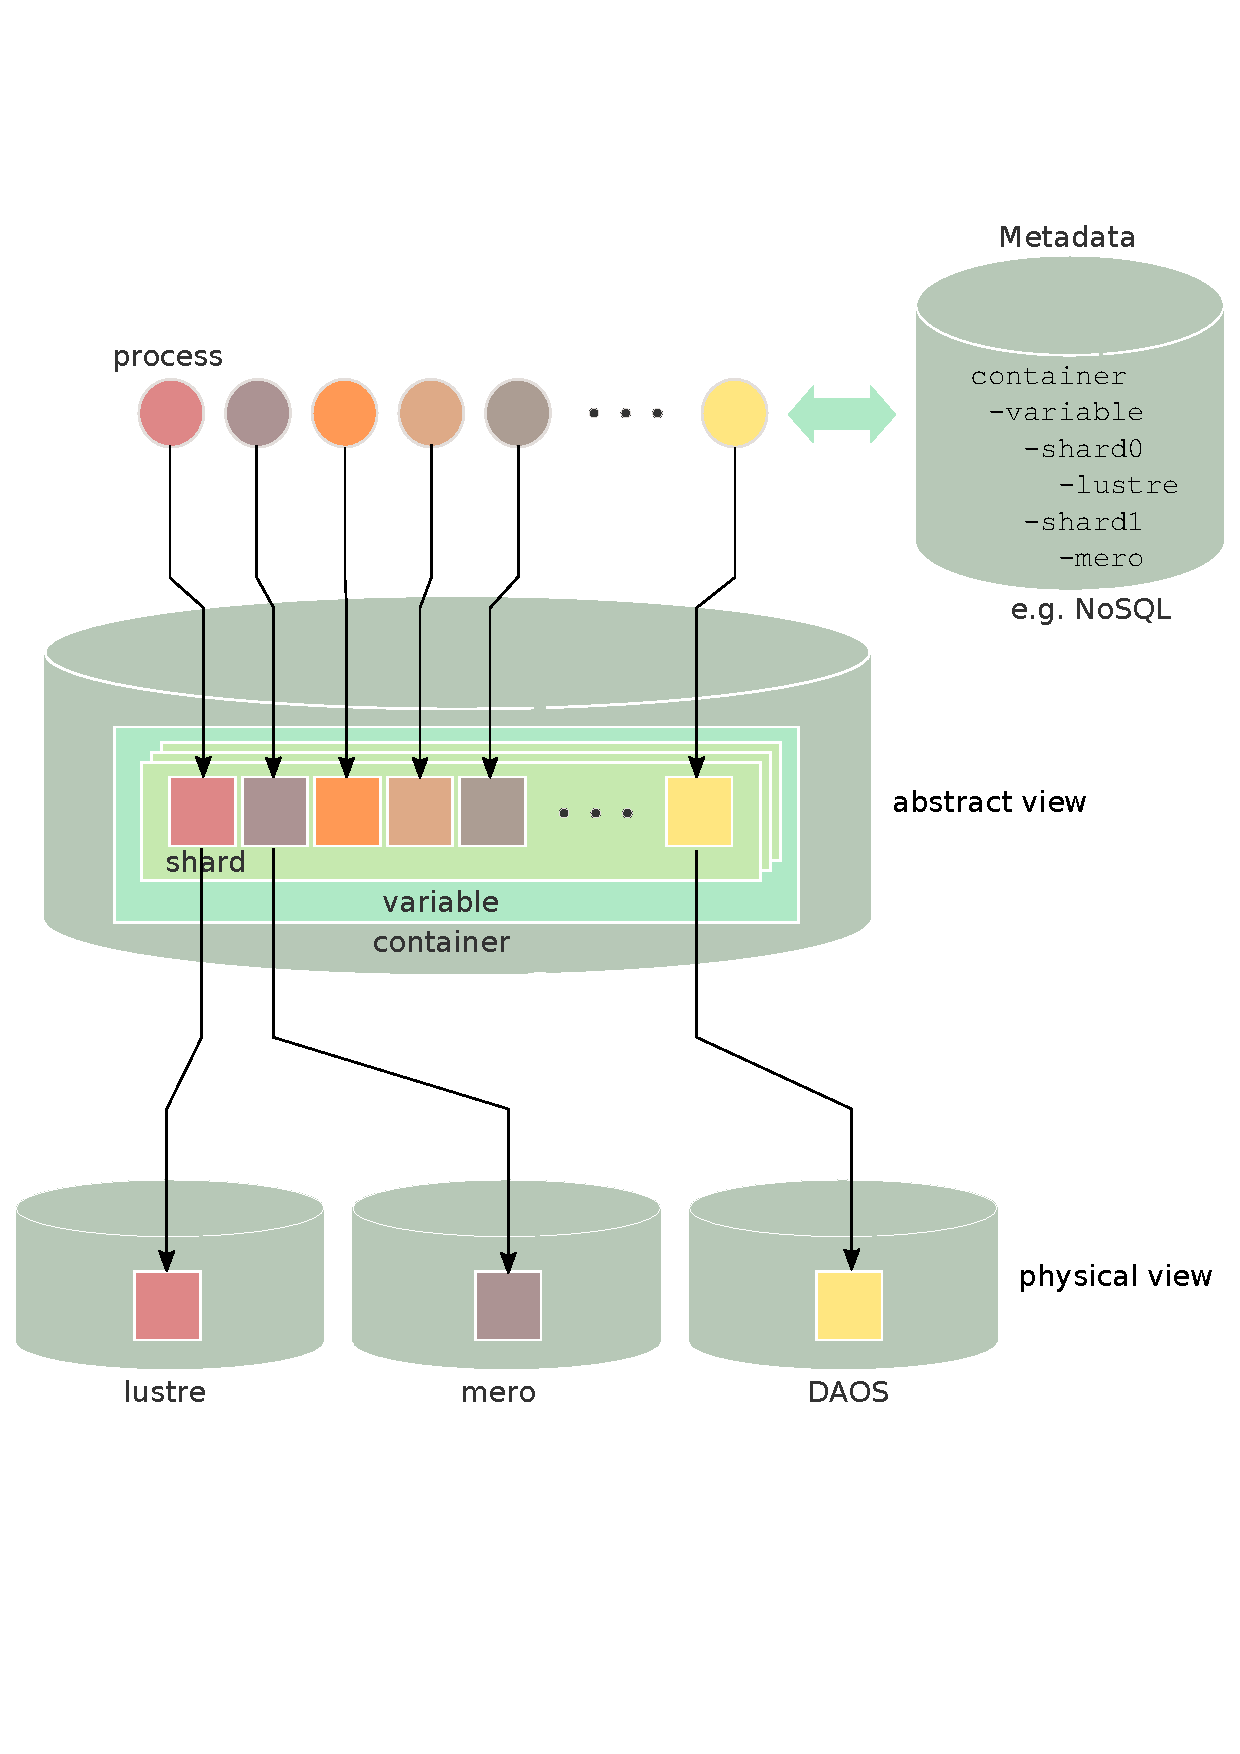
\includegraphics[width=0.7\textwidth]{figures/data-model}
        \caption{}
        \label{fig:data-model};
\end{figure}


%%%%%%%%%%%%%%%%%%%%%%%%%%%%%%%%%%%%%%%%%%%%%%%%%%%%%%%%%%%%%%%%%%%%%%%%%%%%%%%

\subsection{Identifying Resources}
\paragraph{Searching for objects}

In many cases, metadata of logical objects can easily be searched by specifying  query.
API calls will be translated to the internal metadata storage.
An example query is shown in \Cref{lst:extendedSearch}.

\begin{tcbcode}[label={lst:extendedSearch}]{Advanced object search}
\begin{lstlisting}
{ $and : [ 
  { "domain.longitude": { "$gt" : -40, "$lt" : -10 } },
  { "domain.latitude" : { "$gt" : 90}},
  { "domain.time"     : { "$gt" : datetime(2001, 11, 01)} },
  { "info.model.name" : "my model" },
  { "info.environment.system" : "mistral" }
]}
\end{lstlisting}
\end{tcbcode}

An issue are external references, such as the longitude and latitude variables in our example, as they use an index to reference to the specific value indirectly.
One solution to enable search of such variables would be for users to define metadata for a bounding box that will always be included in the metadata and searchable.

Additionally, for convenience of the model, different variables may use alternative coordinate systems or simply use the same metadata field for different meanings.
Luckily in the domain of NWP/climate, there are conventions such as CF that define the metadata.

Identifying all objects that depend on a specific document requires to query the reference field and check if the document ID is part of it.

%%%%%%%%%%%%%%%%%%%%%%%%%%%%%%%%%%%%%%%%%%%%%%%%%%%%%%%%%%%%%%%%%%%%%%%%%%%%%%%



\paragraph{Sealed objects}
Data becomes immutable, once the container is closed...
Useful for referencing to the objects, checksums can then be created and persisted.

\todo{Just thoughts so far?}


\paragraph{Deleting of objects}
When a logical object is about to be deleted, it has to be checked if it is referenced by any other document.
Since the dependencies are stored in each document and this array is indexed, it can be quickly checked if there are any dependencies.
If so, the object cannot be deleted, or the data must be embedded into all referencing documents.
Since this would multiply the storage space for the objects, it is usually favorable to keep the data and the references.

\paragraph{I/O Modes}

The initial version of ESD will support only two modes of access for the data of a variable:
1) write-only append mode; 2) read-only access.
It is not allowed that different independent applications write to the same logical variable.



%%%%%%%%%%%%%%%%%%%%%%%%%%%%%%%%%%%%%%%%%%%%%%%%%%%%%%%%%%%%%%%%%%%%%%%%%%%%%%%
\section{Implications for Developers and End-Users}

For exiting applications the middleware aims to be transparent, albeit not expecting optimal performance exploitation for every use case.


\subsection{MPI Parallel Applications}

This section describes the implications on a existing parallel application that uses one of the supported interfaces such as NetCDF4/HDF5.
The semantics of the API calls will change slightly but mostly in a way that is backwards compatible.

\subsubsection{Open}

Traditionally, when opening a file with NetCDF the filename specifies the location, i.e., an URI where the data resides on a storage system.
We change the notion of the file name to be the descriptor for a virtual container (virtual container descriptor).
The virtual container can be composed of multiple URIs to integrate different variables into one virtual environment on the fly.
Thus, from the reader's perspective it does not matter if data of a model is split into one or multiple physical files; upon read, all those files can be loaded together as if they would already exist in one logical file.

The ESD does not support concurrent read and write scenarios, it is allowed to either write data or to read it (see Epoch).

\todo{extend?}


\subsubsection{Concurrency semantics}

In general, the system is designed for coordinated parallel applications that access data independently of each other.
That means, within one parallel (MPI) application, some kind of coordination happens to allow the shared access to containers, variables and shards.

Data sharing between independent applications is intended to happen after applications completed.
It is not allowed that multiple currently running parallel applications write data to the same variable.
This is considered to be sufficient for most scenarios, e.g., a model produces some output, once the model completed, the produced data is post-processed.
If an application uses the write-only mode to append data to a variable, the concurrent read-only access of the same or independent applications will not immediate see the new data.
Instead, ESD ensures that all changes to the data (and metadata) becomes atomically visible when the logical container is closed by the application.
At this point, all the new data becomes immediately visible to the readers.

Especially in NWP applications it is useful to access intermediate results and start post-processing as soon as possible to minimize the overall delay.
To support this scenario, we provide the concept of Epoch-Semantics to the developers (see below).

Writing data follows the expected semantics for writes but when multiple writers write data to the same variable coordinates, i.e., they overwrite data, the result is undefined.
In fact, applications in which multiple processes write to the same region are considered to be wrong.

Reading data that is available in the container but has been written by a previously terminated application will be returned in the correct fashion.
Reading data that has been written by the same application (i.e., reads after writes) should not happen, as users should use means of communication inside the application to prevent this kind of access pattern.
If such a fine-grained update of data is necessary, again the Epoch-semantics must be used.


\subsubsection{Epoch Semantics}

An epoch is an instant in time chosen by the parallel application. 
Starting with Epoch 0, all processes of the parallel application participating in the I/O have to agree on moving to a new epoch.
This will finalize the outstanding write requests, make the changes durable and publish the information about new data to other applications that registered to read this data.
Writing data to a variable that existed previously will overwrite the data of previous Epochs.
Similarly, if a variable is opened for read/write access, the same application may now read the data from a previous Epoch.
Thus, a read request will never return the data of the current epoch but the merged perspective of all previous Epochs.

Thus, the Epoch semantics is similar to the semantics of transactions but application wide and only one transaction can be active at a given time.

If a parallel applications overwrites data stored in a previously by another application written variable, then this is handled similarly to a new Epoch.

\todo{Figure necessary}

\subsection{Implementing Workflows via Virtual Containers}

This section will demonstrate how multiple post-processing applications can process data that is created from a simulation.
Firstly, we consider the case in which each job in this worklow is run after the previous job completed.

Simulation 
large parallel application


\begin{verbatim}
Virtual container (Input)\footnote{The virtual container provides a hierarchical namespace with names}
- input for simulation
-- grid
--- var 1 
--- var 2
-- configuration.xml

Virtual container (Output)
time series
- var 3
- var 4


Post-processing
few processes

Virtual container (Input)
time series
- var 3

Output
- var 5 (time series)
- var 6: single number
\end{verbatim}


\todo{Figure necessary}

When moving to the Epoch semantics, a time step can be considered as an Epoch.
Whenever one is completed, the post-processing can ingest the new data and process it.

The mapping of the variable name and the actual content is based on the scientific metadata.

An example configuration file for setting up the virtual containers is shown in:

\todo{Configuration file}


%%%%%%%%%%%%%%%%%%%%%%%%%%%%%%%%%%%%%%%%%%%%%%%%%%%%%%%%%%%%%%%%%%%%%%%%%%%%%%%
\subsection{POSIX Tools}

% handle failures/many other things very transparently
% more expressive I/O APIs
% frameworks for HPC application developments that also integrate data services


\subsection{Next Generation Applications}

The ESD middleware could satisfy the need of future applications e.g. for
	in situ/in transit
	workflows
	virtualisation
	parallel in time?
	





%%%%%%%%%%%%%%%%%%%%%%%%%%%%%%%%%%%%%%%%%%%%%%%%%%%%%%%%%%%%%%%%%%%%%%%%%%%%%%%
\subsection{Data Services}

\todo{AS this is in the design chapter, there is many references to related work, but it is not immediately clear what the resulting requirements are.}

\subsubsection{Data Processing}

One of the common themes of research in storage has been to bring specific types of processing closer to the storage.
Obvious first steps in storage-side processing is checking basic data integrity (“did we get all the bytes, and in the
right order?” as well as updating metadata systems (“we have a new file”). The next steps were to automate metadata
extraction in a file-type dependent way, so a process would recognise the file type and apply file-specific checks on
its structural integrity (“is this a well-formed HDF5/PDF/Word document”).  These types of checks are widely used in
production infrastructures.

The next obvious extension to this was twofold: one proposed direction would bring higher level features closer to the
device, to remove the load on filesystems.  For example, in conventional magnetic hard drives one originally had to know
the number of cylinders, sectors, and so on, but LBA vastly simplified supporting hard drives without having to
reconfigure the operating system (or file system), and in a similar vein, hard drives can do their own checking and
management of bad blocks.\todo{It may be worth investigating this further, as LFTS could provide similar benefits for tape?
  or are those benefits irrelevant for the purposes we are discussing here?}

A research extension by SNIA proposed drives that provided direct object storage with metadata, thus bringing some of
the work required by the filesystem into the storage device; the flip side is that the interface would not be full POSIX
but more like an object store.  This particular research, however, never came to production, and we must conclude that
there were not sufficient requirements for it to have a market.

The other direction was in storage management services that would implement programmable storage side workflows, such as
iRODS.  Generally microservices would need to be added in order to support new file types and change the rules, but the
system would be customisable to provide relatively simple workflows which were used to manage metadata but could be
extended to do server side processing.

Grids provide similar features but in a different way, as there is technically no difference between storage-side
processing and user-side processing: they are done using the same mechanisms, but essentially in different data
centres. WLCG operates a tiered model where data is generated at a Tier 0 centre, copied to Tier 1 centres whence it is
copied to Tier 2s (these should not be confused with data centre tiers which are essentially the other way around.)  Raw
processing of data – what we would call storage side processing – is done at the Tier 0 and 1s, with no end user access
at all. End user analysis of data would happen at Tier 2s and 3s, and data which need archiving would be copied back to
the local T1 [diagram]

An alternative approach is to treat the storage as a basic service – like an object store, typically – and let higher
level workflow engines manage the writing and processing of the data as a part of a (loosely coupled) workflow.  This
approach would also work well provided it can get notifications back from the store.  Indeed, CASTOR2 was originally
written on top of LSF, but LSF was removed (around ~2010?) in favour of a bespoke “transfer manager” when it was found
that original versions of CASTOR didn’t scale well with the WLCG workloads10.

(A novel approach is to treat the data structure transparently within the applications, without the requirement to
integrate the data management in the application; see future directions\todo{JJ: check what is available}


\subsubsection{Staging and Caching}

State of the art: ERADAT, the BNL extension of (90PB) HPSS [Yu].  The main question is whether every recall can always
be automated or at which stage would it need operator intervention in order to me maximally efficient?

State of the art – NERSC CORI (2017?) [Dosanjh], NVRAM burst buffers; 28 PB secondary disk (Lustre) supporting data
placement “close” to the CPU; thus a further staging process is required anyway (cf. diagram).  Also JASMIN’s PANASAS
with 15PB (using ET for temporarily staging data in order to free up fast disk)

Note the follow-up requirement on meta-operations on data, e.g. staging, pinning.

\todo{NUMA?}

Is it necessary to generate models for this? Is it useful?  For example, the allocation of drives to each individual
user community, and optionally prioritising recalls.

Could the same be applied for other types of file operations that are scheduled, such as replication and integrity
checking.  It would be useful to do opportunistic operations: if a tape (resp. collection) is mounted
(resp. fetched/unpacked), take the opportunity to act on other collections (files/objects), instead of waiting for their
scheduled operation.



%%%%%%%%%%%%%%%%%%%%%%%%%%%%%%%%%%%%%%%%%%%%%%%%%

\chapter{Architecture Description} 
% https://en.wikipedia.org/wiki/Software_architecture_description

\begin{chapterIntro}
We use the 4+1 view model of architecture according to Philippe Kruchten. 
% http://www.cs.ubc.ca/~gregor/teaching/papers/4+1view-architecture.pdf




To meet the aforementioned challenges, we have designed the \textit{Earth System Data (ESD)} middleware, which:


\begin{enumerate}
	\item can understand application data structures and scientific metadata, letting us expose the same data via different APIs;
	\item can map data structures to different storage backends with different performance characteristics based on site specific performance model configuration;
	\item can yield best write performance via optimized data layout schemes that utilize elements from log-structured file systems;
	\item can provide relaxed access semantics, tailored to scientific data generation for independent writes, and;
	\item 
% 5) semantic views enable to open various collections of data as one virtual container, thus, relieving the issues of hierarchical namespaces and the definition of the scope of a file.
% Note item 5 below should be 6 when 5 above is uncommented
includes a FUSE module which will provide backwards compatibility through existing file formats with a configurable namespace based on scientific metadata.
\end{enumerate}



Together these allow storing small and frequently accessed data on node-local storage, while serializing multi-dimensional data onto multiple storage backends -- providing fault-tolerance and performance benefits for various access patterns at the same time.  Compact-on-read instead of garbage collection will additionally optimize and replicate the data layout during reads via a background service. Additional tools allow data import/export for exchange between sites and tape archives.
% the middleware to use the structural information to optimize workflow performance. 
%\item Services to import/export from/to portable formats on the system boundary / tape archive, 
%\item Configuration file
\end{chapterIntro}


\section{Logical View} % is concerned with the functionality that the system provides to end-users.


The general architecture of the ESD middleware is shown in \Cref{fig:architecture}. 
\todo{extend?, small guide to the chapter?}

\begin{figure}
\centering
\vspace*{-1em}
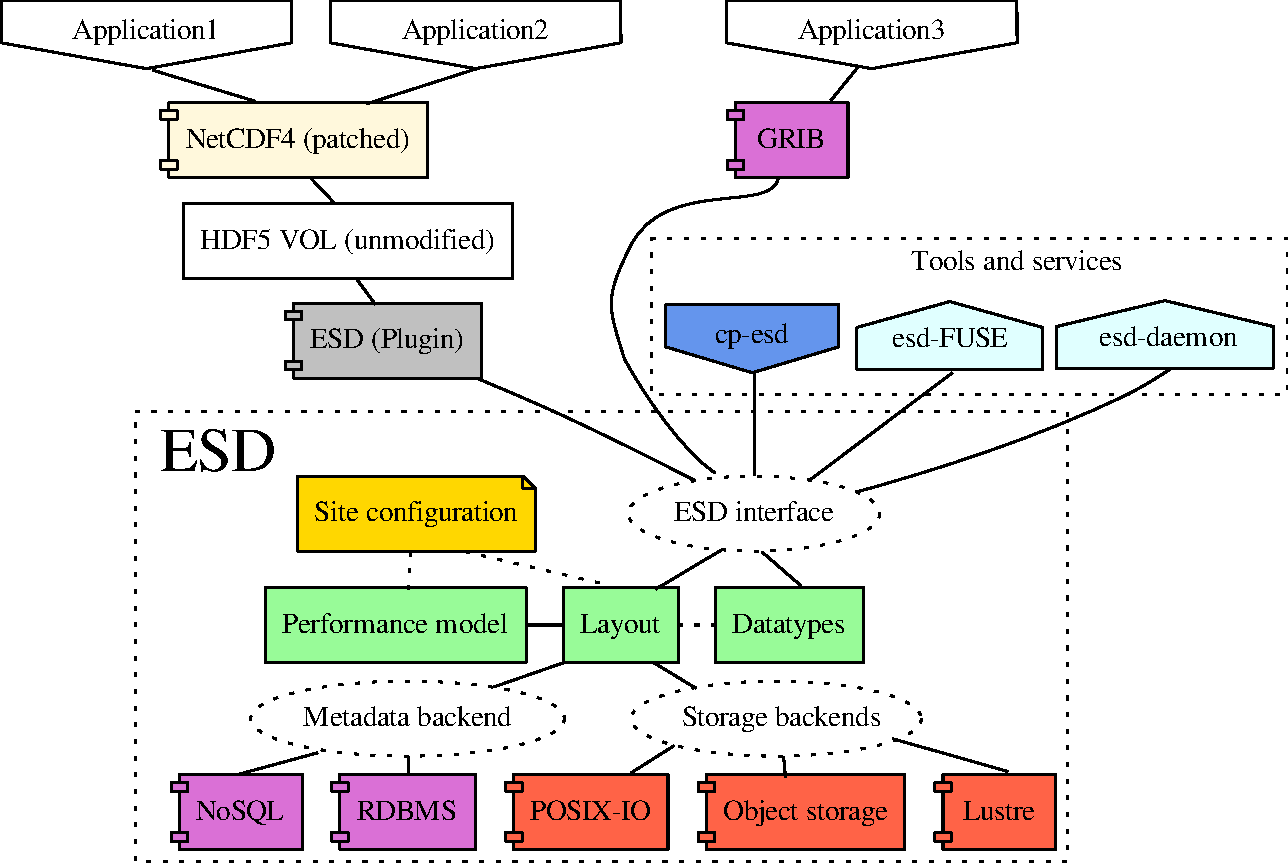
\includegraphics[width=0.98\columnwidth]{figures/architecture-backend}
\vspace*{-0.7em}
\caption{Architecture overview}
\label{fig:architecture}
\vspace*{-1em}
\end{figure}
%While we consider these tools within the design, we won't implement all of them in the scope of the ESiWACE project.

%%%%%%%%%%%%%%%%%%%%%%%%%%%%%%%%%%%%%%%%%%%%%%%%%%%%%%%%%%%%%%%%%%%%%%%%%%%%%%%
\subsection{Interface}
This represents the API exposed to other libraries and users. The API will be independent from the specific I/O backend used to store the data and will support structured queries to perform complex data selections in the variables. The API will be able to support the complex workflows of future applications, while backward compatibility with legacy codes will be provided through a FUSE module. The definition of the ESD interface is out of the scope of this document.

%%%%%%%%%%%%%%%%%%%%%%%%%%%%%%%%%%%%%%%%%%%%%%%%%%%%%%%%%%%%%%%%%%%%%%%%%%%%%%%
\subsection{Datatype Component}
The datatype component will provide native ESD middleware datatypes that can be used by users or other libraries to describe data points inside variables. We follow the approach pursued by the HDF5 library, that is, we provide a set of native datatypes and a basic set of datatype constructors that can be used to build custom derived datatypes. 

%\begin{longtable}{| >{\centering\arraybackslash} m{5.5cm} | >{\centering\arraybackslash} m{6cm} |}\hline\hline
%        \cellHeader Datatype & \cellHeader Description \\ \hline
%        \centering \small ESD\_TYPE\_CHAR & \small 8-bit character \\ \hline
%        \caption{ESD Datatypes}
%        \label{table: esd-type}
%\end{longtable}

%\begin{longtable}{| >{\centering\arraybackslash} m{5.5cm} | >{\centering\arraybackslash} m{6cm} |}\hline\hline
%        \cellHeader Type Constructor & \cellHeader Description \\ \hline
%        \centering \small - & \small - \\ \hline
%        \caption{ESD Datatype Constructors}
%        \label{table: esd-constr}
%\end{longtable}

\todo{What type of datatypes are supported? In principle the ESD can support NetCDF and HDF5 by providing the same datatypes as for HDF5. Are these enough? Need to be extended to support some other type?}.

%%%%%%%%%%%%%%%%%%%%%%%%%%%%%%%%%%%%%%%%%%%%%%%%%%%%%%%%%%%%%%%%%%%%%%%%%%%%%%%
\subsection{Layout Component}
The layout component allows the middleware to store pieces of data on different backends depending on specific site configuration contained in the performance model. The layout component in this case takes responsibility for generating additional technical metadata describing data placement and for storing it in the appropriate metadata backend (i.e. MongoDB). A more detailed description of what technical metadata is, is given in the rest of this section.

%%%%%%%%%%%%%%%%%%%%%%%%%%%%%%%%%%%%%%%%%%%%%%%%%%%%%%%%%%%%%%%%%%%%%%%%%%%%%%%
\subsubsection{Adaptive Data Mappings}
The typical storage mapping for scientific data format libraries is the file (linear sequence of bytes organized following the POSIX file system representation, i.e. inodes and blocks). Information is translated into a linear array of bytes in the file system using appropriate schemas. Since the data model defined by the data format library can contain complex hierarchies and attributes besides raw data, the final file will contain additional scientific metadata that needs to be accessed using the POSIX-IO data interface (e.g. \texttt{read()} and \texttt{write()}) instead of the file metadata interface (e.g. \texttt{stat()}, \texttt{lookup()}). This makes the storage model adopted by data format libraries incompatible with the typical parallel file system organization, in which metadata and data are splitted apart and assigned to different services for optimal performance. Additionally, new storage system paradigms have emerged in the last years in which files are organized in a flat namespace (e.g. object storage), removing the restrictions imposed by metadata operations like namespace traversal of POSIX file systems. Hierarchical organization can be still achieved using other dedicated storage representations like key-value stores, at the expense of reduced POSIX semantic.

There is therefore a necessity for more flexible data mappings that can take advantage of an increasing number of storage and backend alternatives, improving access efficiency at the same time. There are two different approaches to this problem: the first is to develop a new data mapping schema for every storage backend. This is the solution adopted by the HDF5 library (through the virtual file and the virtual object layers) in which multiple storage backends can be employed by developing a corresponding plugin that contains the right mapping schema. The obvious limitation of this solution is that once the user has selected a certain backend for a file, this cannot be changed without migrating the whole file to another backend. The second approach is more flexible and consists in making the storage backend selection adaptive. This has the advantage of enabling backend storage selection on the fly depending upon the type of data being stored or a set of user/system defined parameters (e.g. list of data placement policies satisfying certain requirements of quality of service).

Our proposed solution is to integrate the adaptive data mappings capabilities just discussed in the layout component of the ESD middleware. The middleware will understand the scientific metadata of other relevant data format libraries and will be able to use multiple storage backends at the same time to store and retrieve different pieces of data. To support multiple formats the datatype component in the ESD middleware will expose a datatype interface similar to the one available in HDF5 (described in Section~\ref{sec: data-formats}). Additionally, the middleware will add significant metadata to be used in the life cycle management and sharing of data. This can include semantic metadata describing which data is needed and how it is going to be used, the required level of resilience, etc. In this context, some metadata can be automatically generated by the middleware or defined by the user and passed to the middleware through an apposite interface (that will be part of the ESD exposed interface).

Legacy codes will have access to data using a familiar POSIX interface exported through an ESD FUSE module. The FUSE module will communicate with the ESD middleware to access data and export it to users using a namespace representation. The mapping schema definition for mapping data between the storage representation and the namespace will be done later in the project.

Another important aspect to consider when talking about adaptive data mappings is the storage tiering, that is, how many levels of storage there are in the system. Historically, HPC applications have relied on parallel file systems as first tier to store and retrieve their data. Besides the parallel file system, most high-end clusters have a second level of archival storage to which data is migrated from the parallel file system using a hierarchical storage manager. Nowadays compute nodes have access to local storage (typically a block device formatted with a local file system) and with the emergence of new storage technologies, such as non-volatile memories, permanent byte addressable memory. The ESD middleware should be able to exploit these local storage resources to implement prefetching strategies (read patterns) and burst buffers (write patterns).

%In the specific case of Mero (Seagate object store system), which represents one of the possible storage backends that has to be supported by the ESD middleware, hierarchical and semantic metadata can be stored in the key-value store service while array data can be stored into objects. In fact, we can think about using more than one object per dataset. This is particularly useful with chunking since every chunk in the dataset can be mapped to a different object, making parallel access to different data units possible without any need for I/O coordination (no false sharing is possible in this case). Of course, I/O coordination still needs to be provided when multiple processes access the same dataset and chunking is not enabled. In this case the ROMIO library already provides a collective I/O implementation that can be reused by the ESD middleware. Whenever needed, false sharing of data can also be avoided by using `persistent file realm' like mechanisms\footnote{This mechanism allows a certain file portion to be assigned to a specific process in the application and makes this assignment persistent across multiple data accesses.}.

%\todo{Giuseppe: you had a very good document on this already can add something here}

%Goal of the dynamic mapping is to create a hierarchical namespace based on the available metadata.
%It is based on the search for objects.
%With the help of FUSE, these mappings can be created based on a user configuration upon mount-time (supports user mounts).
%Inaccessible data, i.e., where the permissions are not sufficient, can be hidden from the namespace.

%An example mapping could be:
%“v.info.model/v.info.environment.date/v.info.experiment.tags/v.info.name <as NC4>”.
%This would show a single NetCDF4 file for each variable.
%If a variable is attached to various tags, then it is shown for each of them.

%“v.info.model/v.info.environment.date/v.domain.time/v.info.name <as NC4>”.
%Would show one file per timestep.

%How to resolve ambiguity?

%Existing containers can also be directly mapped, showing the input and output variables similarly:
%“<c.\_id>/<c.directory>”


%The storage should now how the logical data space maps to physical positions in memory or storage.
%If the storage backends have this knowlege, they can run local operations on the data.

%Alternatives:
%Triangular grid (locally refined), somehow mapped from user-space to a 1D structure which gets mapped to the storage. (Traditional approach)

%Application(data structure) - Mapping - Middleware - Mapping (byte array) - Storage API - Storage backend

%or:

%Application - Middleware - Storage API - Mapping - Storage backend

%Use sth. like MPI datatypes to descripe memory (in the application)
%Add metadata to describe the meaning / semantics, additional gain: resilience because we know which data to replicate to put into triple ECC ...
%Add hints how the data is used / will the used in the future

%Avoid redundant descriptions of memory / storage.
%Users stores a 3D field, it is clear which storage location is responsible for [x,y,z]
%How to store triangles etc.

%Why not store code as description?
%- describes neighborhood? 

%Coordinates? Universal coordinates, application coordinates?

%VTK? haben diverse Datenstrukturen hierfür.


%Separation of concerns...

%Missmatch of Chunks size and application domain

%false sharing

%Pointer Datentyp: strong ptr, weak ptr.
%like Boost usw.


%NVRAM

%%%%%%%%%%%%%%%%%%%%%%%%%%%%%%%%%%%%%%%%%%%%%%%%%%%%%%%%%%%%%%%%%%%%%%%%%%%%%%%
\subsubsection{Performance Model}
The performance model characteristics are not clear at this point in time. Nevertheless, we have defined this component in the
ESD middleware so we can use performance parameters to drive data placement in the appropriate storage backend.

%%%%%%%%%%%%%%%%%%%%%%%%%%%%%%%%%%%%%%%%%%%%%%%%%%%%%%%%%%%%%%%%%%%%%%%%%%%%%%%
\subsubsection{Technical Metadata}
Besides scientific metadata, the dynamic mapping of data to storage backends requires further metadata that must be managed.
To distinguish technical metadata from scientific metadata, an internal namespace is created.
Relevant metadata is shown in \Cref{tbl:additionalTechnicalMetadata} for shards, variables and containers, respectively.

Metadata can be optional (O) or mandatory (M), and either is created automatically or must be set manually via the APIs.
Automatic fields cannot be changed.
Some of the data can be automatically inferred if not set manually, but manual setting may allow further optimizations.

Some of the metadata is used on several places, for example, information about the data lineage might be used to create several output variables.
In our initial implementation, the metadata is stored redundantly as this: 
1) simplifies search; 2) enables us to restore data on corrupted storage systems by reading the metadata; 3) reduces contention and potentially false sharing of metadata.
An implementation might decide to reduce this by utilizing a normalized schema.

References is the list of objects that are directly used by this object, e.g., other variables that are used to define the data further.

\begin{table}
\begin{subtable}[t]{\textwidth}
\begin{tabular}{llll}
Metadata & Field & Creation & Description\\
\hline
Domain   & M & Auto & The subdomain this data covers from the variable\\
Type     & M & Auto & The (potentially derived) datatype of this shard\\
Variable & M & Auto & The ID of the variable this data belongs to\\
Storage  & M & Auto & The storage backend used and its options\\
References & M & Auto & A list of objects that are referenced by this data\\
Sealed   & M & Auto & A sealed shard is read-only\\
\end{tabular}
\caption{For a shard}
\end{subtable}

\begin{subtable}[t]{\textwidth}
\begin{tabular}{llll}
Metadata & Field & Creation & Description\\
\hline
Domain      & M & Manual & Describes the overall domain\\
Type   	    & M & Manual & The (potentially derived) datatype\\
Info   	    & M & Manual & The scientific metadata of this document\\
References  & M & Auto & A list of objects that are referenced by this data\\
Permissions & M & Auto/Manual & The owner and permissions \\
Shards      & M & Auto & The list of shard objects for this variable\\
Sealed      & M & Auto & A sealed variable is read-only\\
\end{tabular}
\caption{For a variable}
\end{subtable}

\begin{subtable}[t]{\textwidth}
\begin{tabular}{llll}
Metadata & Field & Creation & Description\\
\hline
Owner    & O     & Manual   & The owner of this file view (see the permission model)\\
Info     & O     & Manual   & Additional scientific metadata for this view\\
Directory & O    & Manual   & Contains a mapping from names to variables\\
Environment & O  & Automatic & Information about the application run\\
Permissions & M & Auto/Manual & The owner and permissions \\
References  & M & Auto & A list of objects that are referenced by this data.
\end{tabular}
\caption{For a container}
\end{subtable}
\caption{Excerpt of additional technical metadata}
\label{tbl:additionalTechnicalMetadata}
\end{table}


\paragraph{Example}

This example illustrates data of a predictive model could be stored on the system and the resulting metadata.
The dimensionality of the underlying grid is fixed.

The application uses the following information to drive the simulation:
\begin{itemize}
 \item Timerange: the simulated model time (from a starting datetime to the specified end)
 \item Longitude/Latitude: 1D data field with the coordinates [float]
 \item Temperature: Initial 2D field defined on (lon, lat)
\end{itemize}
A real model would use further parameters to estimate the temperature but these are sufficient to demonstrate the concepts.
This information is either given as parameter to the simulation or read from an input (container).
A mixture of both settings is possible.


The application produces the following output:
\begin{itemize}
  \item Longitude/Latitude: 1D data field with the coordinates [float]
  \item Model time: the current datatime for the simulation
  \item Temperature: 2D field defined on (lon, lat, time) [float], containing the precise temperature on the coordinates defined by lon and lat for the given timestep
  \item AvgTemp: 1D field defined on (time) [float]; contains the mean temperature for the given time
\end{itemize}


Upon application startup, we create a new virtual container that provide links to the already existing input.
In \Cref{lst:mongoContainer}, the metadata for the container is shown, after the application is started.
We assume it has used the APIs to provide the information (input, output, scientific metadata).
In this example, we explicitly define the objects used as input; it is possible to also define
the input as an already existing container.
It is also possible to define the input a-priori if the objectIDs are known / looked up prior application run.
The intended output variables could be given with their rough sizes.
This would allow the scheduler to pre-stage the input and ensure that there is enough storage space available for the output.
The environment information is inferred to the info object but can be changed from the user.

\todo{How does this align with the use case chapter?}
\todo{Do the examples deserve a clear seperation.. so that general abstractions and vague requirements hidden in a example are clearer?}

\begin{tcbcode}[label={lst:mongoContainer}]{JSON document describing the container}
\begin{lstlisting}
"_id" : ObjectId(".."),
"directory" : {
  "input" : { 
    "longitude" : ObjectId(".."),
    "latitude" : ObjectId(".."), 
    "temperature" : ObjectId("..") 
   },
  "output" { 
     "temperature" : ObjectId(".."),
     "avgTemp" : ObjectId("..")
   }
},
"info" : {
  "model" : { "name" : "my model", "version" : "git ...4711" },
  "experiment" : { 
    "tags"        : ["simulation", "poisson", "temperature"]
    "description" : "Trivial simulation of temperature using a poisson process"
  },
},
"environment" : {  
  "date"  : datetime(2016, 12, 1), 
  "system" : "mistral", 
  "nodes" : ["m[1-1000]"] 
},
"permissions" : {
  "UID"  : 1012,
  "GID"  : 400,
  "group" : "w", # allows read also
  "other" : "r"
},
"references" : {
  [ all links to used object IDs from input / output ]
}
\end{lstlisting}
\end{tcbcode}

The metadata for a single variable is build based on the information available in the container and additional data provided by the user.
An example for the temperature variable is shown in \Cref{lst:mongotemperature}.
When describing the domain that is covered by the variable, there are two alternatives:
1) a reference to an existing variable is embedded and the minimum / maximum value is provided.
This allows to reuse descriptive information as data has to be stored only once. Min and max describe the multidimensional index of the subdomain in the variable that is actually referenced;
2) data becomes embedded into the file. This option is used when the size of the variable is small.

An advantage of option 2) is that searches for data with a certain property do not require to lookup information in additional metadata.

Similarly, information about the data lineage (history) can originally be inferred from the objects linked in the directory mapping.
The metadata of the referenced object must be copied, if the original object is removed.

\begin{tcbcode}[label={lst:mongotemperature}]{JSON document for temperature}
\begin{lstlisting}
"_id" : ObjectId("<TEMPID>"),
"sealed" : true,
"domain" : [
    "longitude" : [ "min" : 0, "max" : 359999, "reference" : ObjectId("..") ],
    "latitude" : [ "min" : 0, "max" : 179999, "reference" : ObjectId("..") ],
    "time" : [ datetime(...), datetime(...), ... ]
  ],
"type" : "float",
"info" : {
  "convention" : "CF-1.0",
  "name" : "temperature",
  "unit" : "K",
  "long description" : "This is the temperature",
  "experiment" : { 
    "tags"        : ["simulation", "poisson", "temperature"]
    "description" : "Trivial simulation of temperature using a poisson process"
  },
  "model" : { "name" : "my model", "version" : "git ...4711" },
  "directory" : {
	"input" : {
	  "longitude" : ObjectId("<LONID>"),
	  "latitude" : ObjectId("<LATID>"), 
	  "temperature" : ObjectId("<TEMPID>")
	}  
  },
  "environment" : {
    "date"    : datetime(2016, 12, 1),
    "system" : "mistral",
    "nodes"  : ["m[1-1000]"]
  },
  "history" : [
    #The history for the inputs, if the data lineage must be embedded
    ObjectId(<LONID>) : [
      # Assume LONID does not exist any more
    ],
  ]
},
"permissions" : {
  "UID"  : 1012,
  "GID"  : 400,
  "group" : "w", # allows read also
  "other" : "r"
},
"references" : {
  [ all links to used object IDs ]
},
"shards" : [
  ObjectId(<SHARD1 ID>), 
  # For a sealed object, the domains of its shards can optionally be embedded:
  { "reference" : ObjectId(<SHARD2 ID>), "storage" : ... , "domain" },   
  ObjectId(<SHARD3 ID>),
  ObjectId(<SHARD4 ID>)
]
\end{lstlisting}
\end{tcbcode}

The variable is split into multiple shards; metadata for one of them is shown in \Cref{lst:mongotemperatureshard}.
Since we assume domain decomposition in the application, the longitude and latitude variables are now only partially stored in a shard.
In the example, we assume two processes create one shard each and the surface of the earth is partitioned into four non-overlapping rectangles.

\begin{tcbcode}[label={lst:mongotemperatureshard}]{JSON document for a shard of the temperature variable}
\begin{lstlisting}
"_id" : ObjectId("<SHARD1 ID>"),
"sealed" : true,
"variable" : ObjectId("<TEMPID>"),
"type" : "float",
"domain" : {
    "longitude" : [ "min" : 0, "max" : 179999, "reference" : ObjectId("..") ],
    "latitude" : [ "min" : 0, "max" : 89999, "reference" : ObjectId("..") ],
    "time" : [ datetime(...), datetime(...), ... ]
  },
"storage" : {
    "plugin" : "pfs",
    "options" : {
      "path" : "/mnt/lustre/testdir/file1",
    },
    "serialization" : "row-major"
  },
"references : [
  ObjectId("<TEMPID>"),
  ObjectId(".."),
  ObjectId("..")
]
\end{lstlisting}
\end{tcbcode}

%%%%%%%%%%%%%%%%%%%%%%%%%%%%%%%%%%%%%%%%%%%%%%%%%%%%%%%%%%%%%%%%%%%%%%%%%%%%%%%
\subsection{Data/Metadata Backend Drivers}
A prototypical metadata backend will be realized using MongoDB.
Advantages of using MongoDB are that it scales horizontally with the number of servers, provides fault-tolerance and that the document model supports arbitrary schemas.

\todo{stub}

To illustrate the applied mapping, we use a subset of our NetCDF metadata described in \Cref{sec:netcdfDataMapping}.
The excerpt is given in \Cref{lst:NetCDF-data-map}.
The mapping of a single logical variable is examplarily described in


\begin{tcbcode}[label={lst:NetCDF-data-map}]{NetCDF metadata for one variable}
\begin{lstlisting}
dimensions:
	longitude = 480 ;
	latitude = 241 ;
	time = UNLIMITED ; // (1096 currently)
variables:
	float longitude(longitude) ;
		longitude:units = "degrees_east" ;
		longitude:long_name = "longitude" ;
	float latitude(latitude) ;
		latitude:units = "degrees_north" ;
		latitude:long_name = "latitude" ;
	int time(time) ;
		time:units = "hours since 1900-01-01 00:00:0.0" ;
		time:long_name = "time" ;
		time:calendar = "gregorian" ;
	short sund(time, latitude, longitude) ;
		sund:scale_factor = 0.659209863732776 ;
		sund:add_offset = 21599.6703950681 ;
		sund:_FillValue = -32767s ;
		sund:missing_value = -32767s ;
		sund:units = "s" ;
		sund:long_name = "Sunshine duration" ;
		
// global attributes:
		:Conventions = "CF-1.0" ;
		:history = "2015-06-03 08:02:17 GMT by grib_to_netcdf-1.13.1: grib_to_netcdf /data/data04/scratch/netcdf-atls14-a562cefde8a29a7288fa0b8b7f9413f7-lFD4z9.target -o /data/data04/scratch/netcdf-atls14-a562cefde8a29a7288fa0b8b7f9413f7-CyGl1B.nc -utime" ;
}
\end{lstlisting}
\end{tcbcode}

\todo{citations: WDCC, CERA}

To simplify search and identify data clearly, data services such as the WDCC[TODO] and CERA[TODO], that offer data to the community, request scientists to provide additional metadata.
Normally, such data is provided when the results of an experiment is ingested into such a database.
Example metadata is listed in \Cref{tbl:additionalMetadata}.
In existing databases, the listed metadata is split into several fields, e.g. an address and email for persons, for simplicity only a rough overview is given.
Instead of encoding the history as a simple text field, it could 
indicate detailed steps including the arguments for the commands and versions and transformations to reproduce the data.
This should include for each step, where and the time when it is performed, and the versions of software used.

It is easily imaginable that most of this information could be useful already when the data is created as it simplifies the search and data management on the online storage.
Some of the data fields become only available after the initial data creation, e.g., the DOI.
Potentially the data must be updated / curated after the data is created.

\begin{table}
\begin{tabular}{ll}
Metadata & Description\\
\hline
Project & The scientific project during which the data is created \\
Institute & The institution which conducted the experiment\\
Person &  A natural person; could be a contact, running the experiment \\
Contact & Reference to person or consortium \\
DOI      & A document object identifier; useful for identifying a data publication\\
Topic     & Some information about the topic of the data / experiment \\
Experiment & Description of this particular experiment \\
History & A list with the history and transformations conducted with the data \\
\end{tabular}
\caption{Excerpt of additional scientific metadata}
\label{tbl:additionalMetadata}
\end{table}

%%%%%%%%%%%%%%%%%%%%%%%%%%%%%%%%%%%%%%%%%%%%%%%%%%%%%%%%%%%%%%%%%%%%%%%%%%%%%%%
\subsubsection{Mapping with MongoDB}
Each object in the data model (container, variable, shard) becomes a collection with indices on certain fields.
Multikey indices allow to index array fields such as the references.

%%%%%%%%%%%%%%%%%%%%%%%%%%%%%%%%%%%%%%%%%%%%%%%%%%%%%%%%%%%%%%%%%%%%%%%%%%%%%%%
\subsubsection{Mapping with Mero}\todo{add mero mapping description}
Mero is an Exascale ready Object Store system developed by Seagate and built from the ground up to remove the performance 
limitations typically found in other designs. Unlike similar storage systems (e.g. Ceph and DAOS) Mero does not rely on any other 
file system or raid software to work. Instead, Mero can directly access raw block storage devices and provide consistency,
durability and availability of data through dedicated core components. Like Ceph Mero provides a key-value store component for small 
data and metadata and an object storage for raw data.

The key-value store component in Mero can be used to keep track of containers, corresponding variables and shard inside them.
For example, each container will be represented as index in Mero. Every index will have references to all the contained variables.
Variable are also represented as indices and will contain variable metatada as well as references to shards. Shards in this case
can be stored as different Mero objects or files in other storage backends.


\subsection{Services}

\todo{}

\subsection{Import/Export of Data}

\todo{}

\section{Process View}% : deals with the dynamic aspect of the system, explains the system processes and how they communicate, and focuses on the runtime behavior of the system.

\todo{}

\subsection{Services}

\todo{}

\section{Physical View} % : depicts the system from a system engineer's point of view. It is concerned with the topology of software components on the physical layer, as well as communication between these components.

\todo{}

\subsection{Deployment on DKRZ}

\todo{}

\subsection{Deployment on STFC}

\todo{}

\subsection{Deployment on CMCC}

\todo{}

\section{Development View} %illustrates a system from a programmers perspective and is concerned with software management.

\todo{}







%\section{Data protocols}
%Protocols like S3 and GridFTP, HTTP as data access and transfer protocols; compare (maybe) other research communities.
%Note that protocols may need to support other types of application-data interfaces (cf.\ D4.1), not just data access, so
%one should not narrow it down in general to a single use case.
%How do protocols advertise features and carry metadata (such as permissions) - like FEAT in (Grid)FTP, and HTTP headers
%for permissions --- whole additional protocols built around, or integrated with, data protocols (cf. GSS, TLS).


%\chapter{Current Areas of Research and Future Directions}
%Software defined networking (SDN) and software defined storage? (maybe analogy, compare with the WSRF architecture and
%design? - thinking out loud.)
%Integration of data services closer into the application, cf. BSC's work on persisting data structures in applications.
%Running workflows ``near'' the data, compared to traditional HPC applications.  Simplified domain-specific workflows may
%integrate relatively well with other types of data management workflows (cf. iRODS).





%%%%%%%%%%%%%%%%%%%%%%%%%%%%%%%%%%%%%%%%%%%%%%%%%%%%%%%%%%%%%%%%%%%%%%%%%%%%%%%
\chapter{Summary and Conclusions}

The ESD aids the interests of stakeholders: developers have less burden to provide system specific optimizations and can access their data in various ways.
Data centers can utilize storage of different characteristics.
We expect a working prototype with the core functionality within the next year.  Following work
 will implement and fine-tune the cost model and layout component and provide additional backends.







%%%%%%%%%%%%%%%%%%%%%%%%%%%%%%%%%%%%%%%%%%%%%%%%%%%%%%%%%%%%%%%%%%%%%%%%%%%%%%%
\acknowledgement


%\nocite{*}
\bibliographystyle{alpha}
\bibliography{bibliography.bib}

\end{document}
